\documentclass{article}
\usepackage{color,soul}
\usepackage{amsmath}
\usepackage{amsfonts} 
\usepackage{eqnarray}
\usepackage{bm}
\usepackage{multirow}
\usepackage{graphicx}
\usepackage{booktabs}
\usepackage{comment}
\usepackage{subcaption}
\usepackage{listings}
\usepackage[margin=0.5in]{geometry}

\title{School of Electrical and Computer Engineering\\
Purdue University, WL, IN, USA}
\author{Nahian Ibn Hasan\\
Email: hasan34@purdue.edu\\
PUID: 0032764564\\
ECE66100 - Computer Vission\\
Fall 2022\\
Homework-6}
\date{\today}

\begin{document}
\maketitle
\section{Objective}
In this homework, we will implement image segmentation and contour extraction algorithms. The expected results should show the separation of a foreground object from the background. This homework will require per-image parameter tuning to obtain visually acceptable results.
\section{Theoretical Questions}
Lecture 15 presented two very famous algorithms for image segmentation: The Otsu Algorithm and the Watershed Algorithm. These algorithms are as different as night and day. Present in your own words the strengths and the weaknesses of each. (Note that the Watershed algorithm uses the morphological operators that we discussed in Lecture 14.)
\subsection*{Answer}
\textbf{OTSU Algorithm:}\\
The algorithm is very is easy to implement. when the difference in grayscale level is large between the foreground and background, the algorithm can easily differentiate the objects. When the grayscale level of both foreground and background are very similar, there is not a well defined threshold level that can effectively differentiate the foreground from background.\\
\\
\textbf{Watershed Algorithm:}\\
The algorithm has some intuitive meaning and is very fast. It also generates complete boundaries. Sometimes the image can get over segmenteddue to huge number of local minima.


\section{OTSU Algorithm}
The OTSU algorithm first forms a histogram of the input gray-scale image with a gray scale level from 0 to 255. The probability of each gray level can be calculated as $p_i = n_i/N$, here, $n_i$=number of pixels in the $i^{th}$ graylevel and N is the total number of pixels in the image.Let $k$ be the threshold gray-level that differentiates the foreground from background. Then the probability of foreground and background pixels can be calculated as $w_0=\sum\limits_{i=1}^{k}p_i$ and $w_1=\sum\limits_{i=k+1}^{255}p_i$, respectively. After that, the mean of each class and inter-class variance is calcuted as $\mu_0 = \frac{1}{w_0}\sum\limits_{i=1}^{k}ip_i$, $\mu_0 = \frac{1}{w_1}\sum\limits_{i=k+1}^{255}ip_i$ and $\sigma^2=w_0w_1(\mu_0-\mu_1)^2$. The task is to maximize $\sigma^2$ for different $k$. We ran the above steps for 10 iterations every iteration starts with the foreground image found from the previous step.
\section{Image Segmentation Using RGB Values}
For each channel, the OTSU algorithm is applied and the results from three different channels are logically AND-ed to get the final segmentation.
\section{Image Segmentation using Texture-based Features}
For the image texture, we considered the local variance of each pixel and applied three different widow sizes. After that the three results are stacked to form three channels of the textured image and applied to the OTSU algorithm as the previous section.
\section{Contour extraction}
For contour extraction, we followed a special approach. For each non-zero pixel in the binary mask from OTSU algorithm, we consider it a part of the contour if there is at least one zero pixel in its 8 neighborood.
\section{Hyperparameters}
Number of Iterations in OTSU algorithm = 10\\
Texture Feature = local variance\\
Texture sliding window size, N = image dependent, mentioned in figures in the Result section


\newpage
\section{Results}
\subsection{Image-1}
Foreground = Cat\\
\begin{figure}[!htbp]
     \centering
     \captionsetup[subfigure]{labelformat=empty}
    \subcaptionbox{\large\textbf{a}}{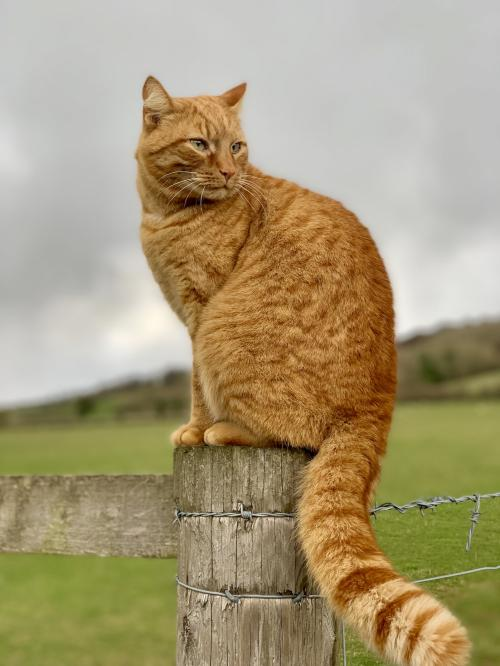
\includegraphics[width=0.19\textwidth]{../Images/cat.jpg}}
    \subcaptionbox{\large\textbf{b}}{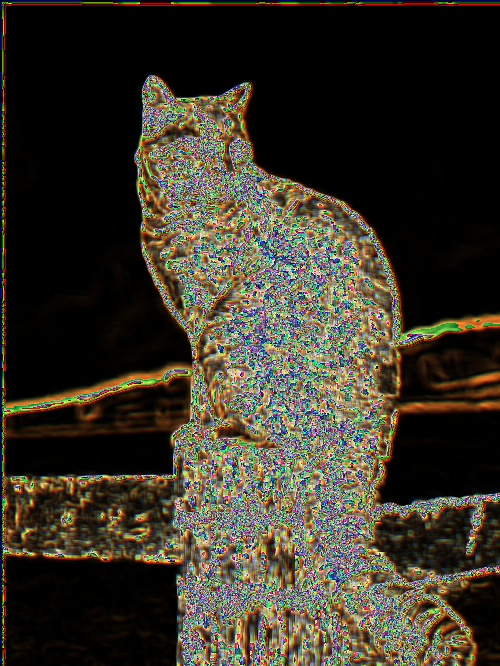
\includegraphics[width=0.19\textwidth]{../My_Code/Output/cat/textures_var_cat.jpg}}
    \caption{(a)Input RGB Image. (b)Textured Image formed by $3\times 3$,$5\times 5$ and $7\times 7$ windowed channels.}
    \label{fig:cat_1}
\end{figure}
\begin{figure}[!htbp]
     \centering
    \captionsetup[subfigure]{labelformat=empty}
    \subcaptionbox{\large\textbf{a}}{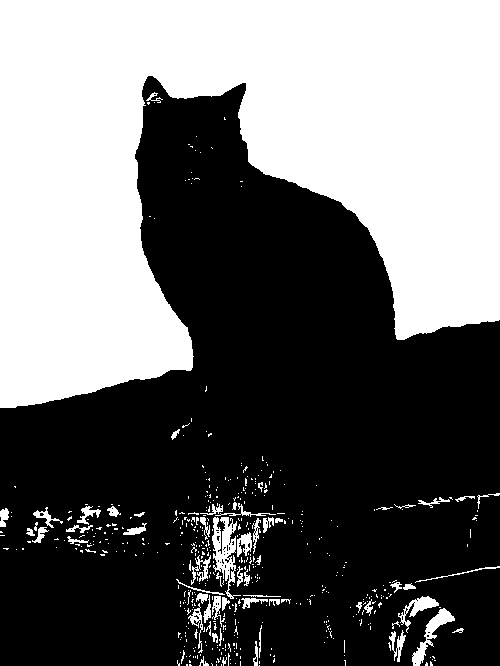
\includegraphics[width=0.19\textwidth]{../My_Code/Output/cat/cat_ch_0_otsu_gray_scale.jpg}}
    \subcaptionbox{\large\textbf{b}}{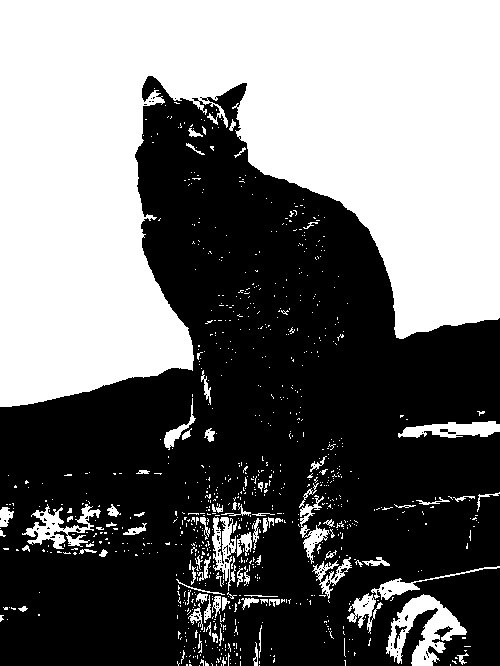
\includegraphics[width=0.19\textwidth]{../My_Code/Output/cat/cat_ch_1_otsu_gray_scale.jpg}}
    \subcaptionbox{\large\textbf{c}}{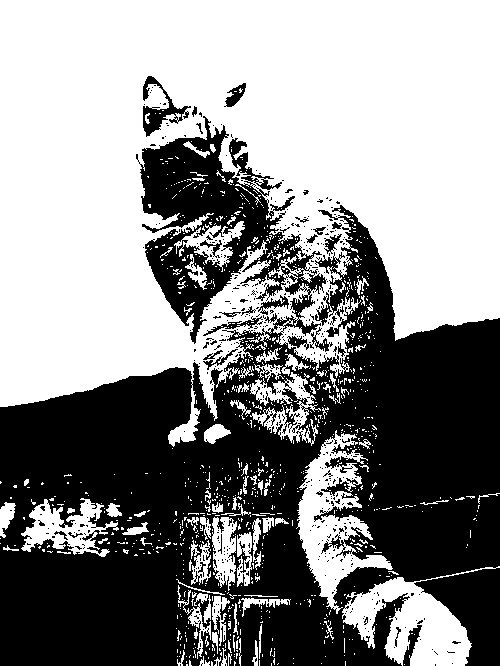
\includegraphics[width=0.19\textwidth]{../My_Code/Output/cat/cat_ch_2_otsu_gray_scale.jpg}}
    \subcaptionbox{\large\textbf{d}}{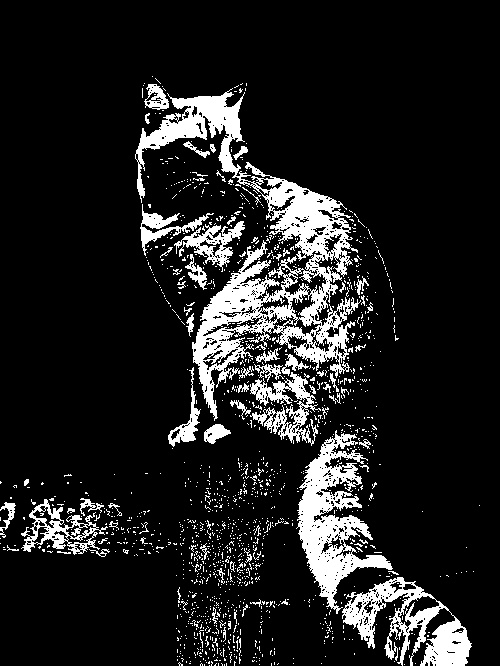
\includegraphics[width=0.19\textwidth]{../My_Code/Output/cat/cat_otsu_RGB.jpg}}
    \subcaptionbox{\large\textbf{e}}{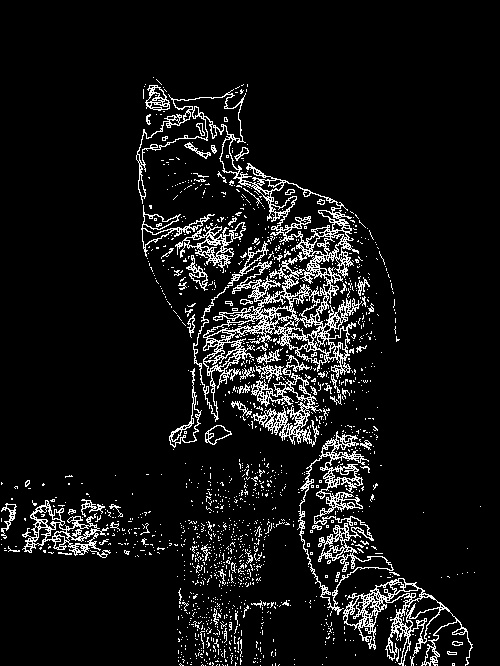
\includegraphics[width=0.19\textwidth]{../My_Code/Output/cat/cat_contour_raw_otsu_RGB.jpg}}
    \caption{RGB-Based Image Segmentation using OTSU Algorithm. Results from channel 1 (a-blue channel), channel 2 (b-green channel) and channel 3 (c-red channel). (d) shows the combined result of all three channels by the operation [AND(R,R-AND(G,B))]. Here, R,G,B are three different channels. (e) shows the extracted contour from the segmented image.}
    \label{fig:cat_2}
\end{figure}
\begin{figure}[!htbp]
     \centering
    \captionsetup[subfigure]{labelformat=empty}
    \subcaptionbox{\large\textbf{a}}{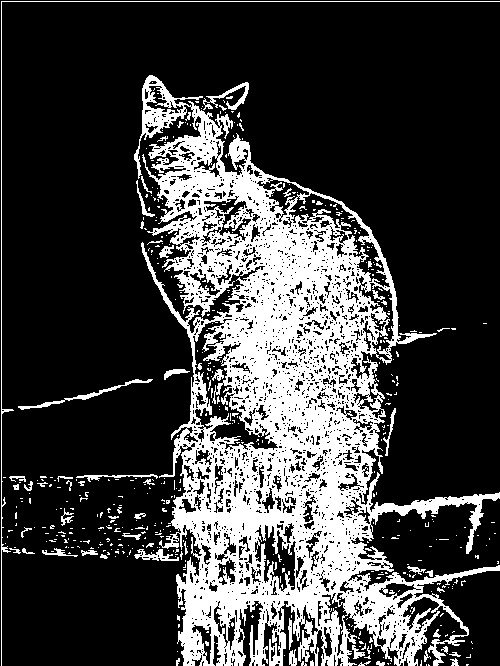
\includegraphics[width=0.19\textwidth]{../My_Code/Output/cat/cat_texture_ch_0_otsu_gray_scale.jpg}}
    \subcaptionbox{\large\textbf{b}}{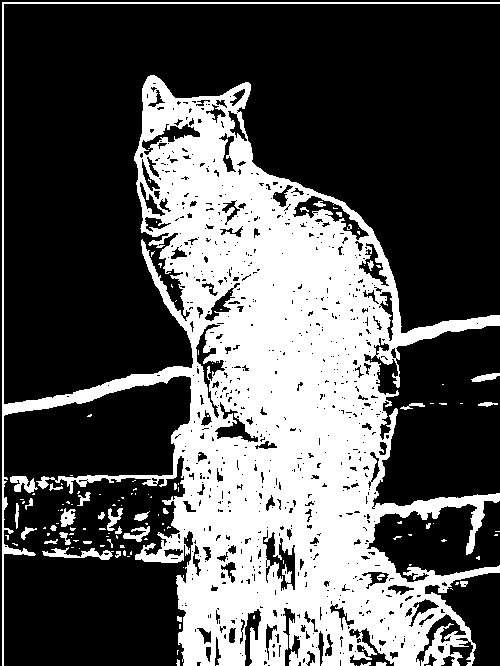
\includegraphics[width=0.19\textwidth]{../My_Code/Output/cat/cat_texture_ch_1_otsu_gray_scale.jpg}}
    \subcaptionbox{\large\textbf{c}}{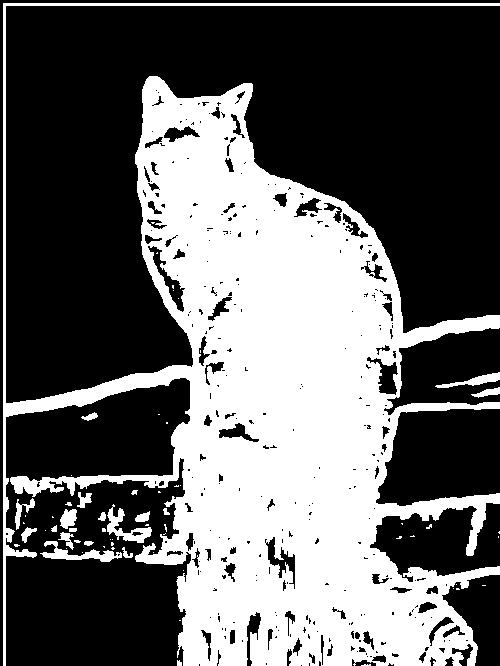
\includegraphics[width=0.19\textwidth]{../My_Code/Output/cat/cat_texture_ch_2_otsu_gray_scale.jpg}}
    \subcaptionbox{\large\textbf{d}}{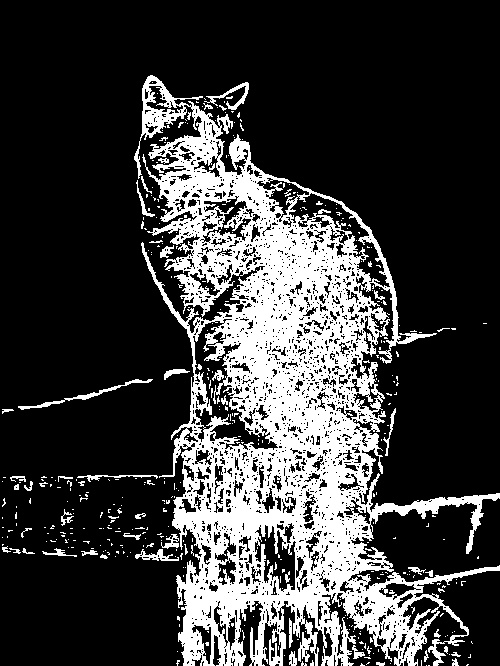
\includegraphics[width=0.19\textwidth]{../My_Code/Output/cat/cat_texture_otsu_RGB.jpg}}
    \subcaptionbox{\large\textbf{e}}{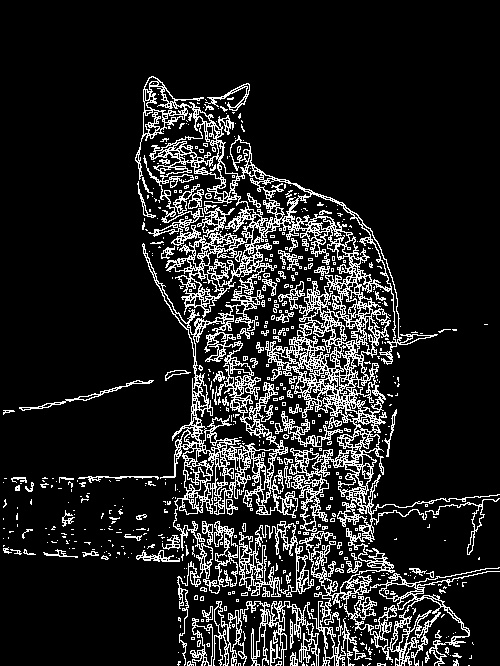
\includegraphics[width=0.19\textwidth]{../My_Code/Output/cat/cat_contour_texture_otsu_RGB.jpg}}
    \caption{Texture-Based Image Segmentation using OTSU Algorithm. Results from channel 1 (a-blue channel), channel 2 (b-green channel) and channel 3 (c-red channel). (d) shows the combined result of all three channels formed by logical AND operation among all masks from all channels. (e) shows the extracted contour from the segmented image.}
    \label{fig:cat_3}
\end{figure}

\newpage
\subsection{Image-2}
Foreground = Car\\
\begin{figure}[!htbp]
     \centering
     \captionsetup[subfigure]{labelformat=empty}
    \subcaptionbox{\large\textbf{a}}{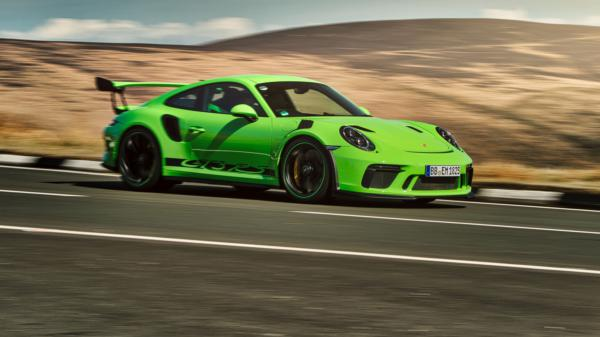
\includegraphics[height=0.15\textwidth, width=0.20\textwidth]{../Images/car.jpg}}
    \subcaptionbox{\large\textbf{b}}{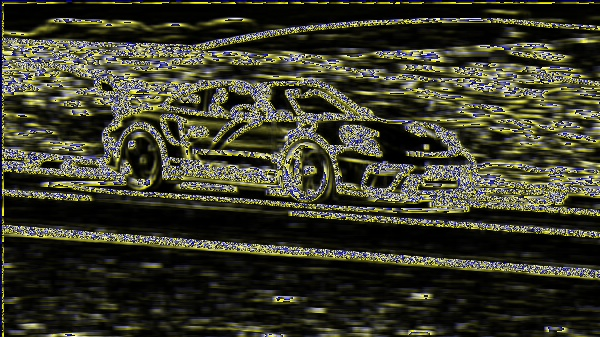
\includegraphics[height=0.15\textwidth, width=0.20\textwidth]{../My_Code/Output/car/textures_var_car.jpg}}
    \caption{(a)Input RGB Image. (b)Textured Image formed by $3\times 3$,$5\times 5$ and $7\times 7$ windowed channels.}
    \label{fig:car_1}
\end{figure}
\begin{figure}[!htbp]
     \centering
    \captionsetup[subfigure]{labelformat=empty}
    \subcaptionbox{\large\textbf{a}}{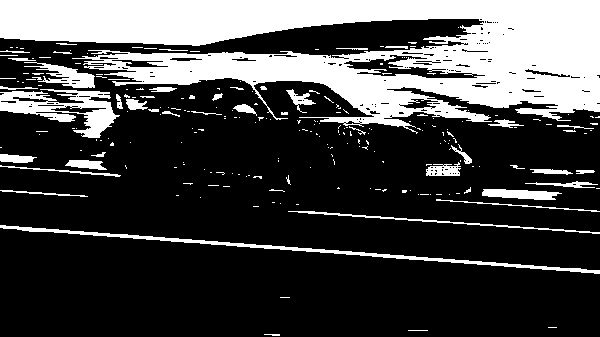
\includegraphics[height=0.15\textwidth, width=0.19\textwidth]{../My_Code/Output/car/car_ch_0_otsu_gray_scale.jpg}}
    \subcaptionbox{\large\textbf{b}}{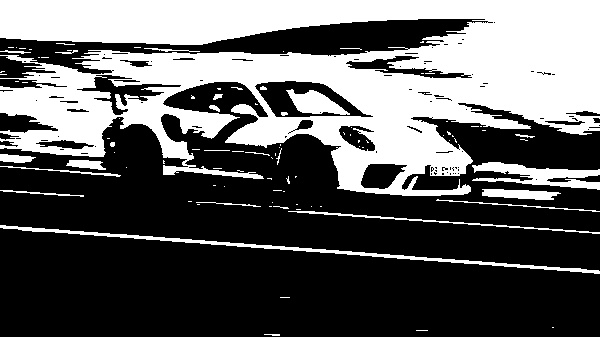
\includegraphics[height=0.15\textwidth, width=0.19\textwidth]{../My_Code/Output/car/car_ch_1_otsu_gray_scale.jpg}}
    \subcaptionbox{\large\textbf{c}}{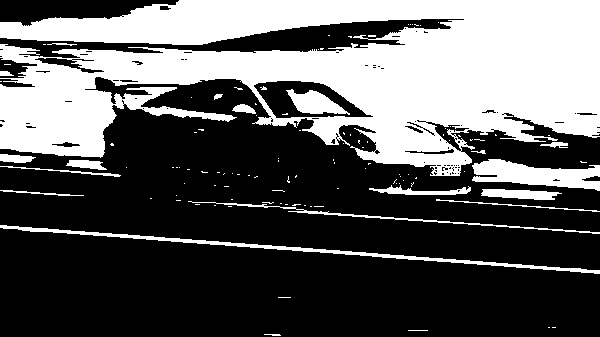
\includegraphics[height=0.15\textwidth, width=0.19\textwidth]{../My_Code/Output/car/car_ch_2_otsu_gray_scale.jpg}}
    \subcaptionbox{\large\textbf{d}}{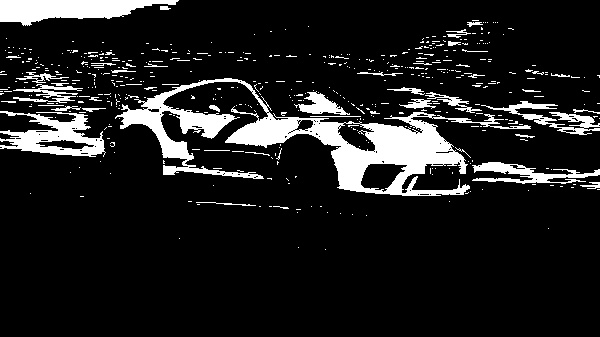
\includegraphics[height=0.15\textwidth, width=0.19\textwidth]{../My_Code/Output/car/car_otsu_RGB.jpg}}
    \subcaptionbox{\large\textbf{e}}{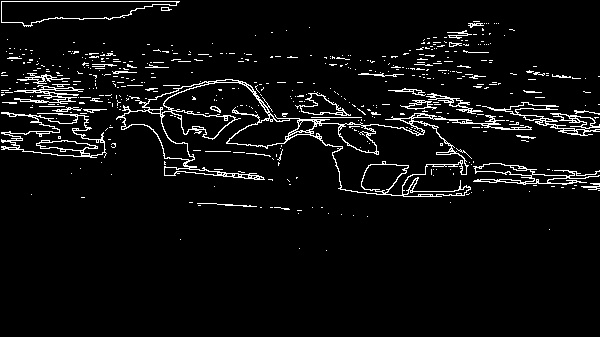
\includegraphics[height=0.15\textwidth, width=0.19\textwidth]{../My_Code/Output/car/car_contour_raw_otsu_RGB.jpg}}
    \caption{RGB-Based Image Segmentation using OTSU Algorithm. Results from channel 1 (a-blue channel), channel 2 (b-green channel) and channel 3 (c-red channel). (d) shows the specially combined result of all three channels by the operation [AND(G,G-AND(R,B))]. Here, R,G,B are three different channels. (e) shows the extracted contour from the segmented image.}
    \label{fig:car_2}
\end{figure}
\begin{figure}[!htbp]
     \centering
    \captionsetup[subfigure]{labelformat=empty}
    \subcaptionbox{\large\textbf{a}}{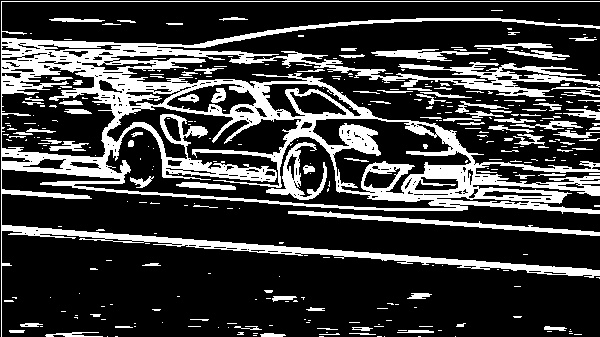
\includegraphics[height=0.15\textwidth, width=0.19\textwidth]{../My_Code/Output/car/car_texture_ch_0_otsu_gray_scale.jpg}}
    \subcaptionbox{\large\textbf{b}}{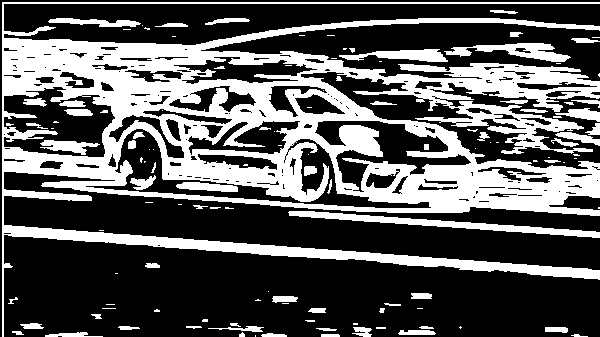
\includegraphics[height=0.15\textwidth, width=0.19\textwidth]{../My_Code/Output/car/car_texture_ch_1_otsu_gray_scale.jpg}}
    \subcaptionbox{\large\textbf{c}}{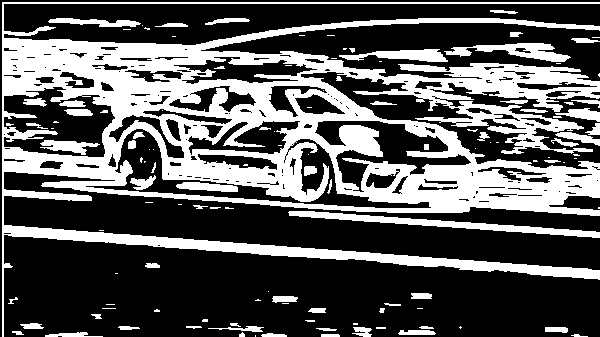
\includegraphics[height=0.15\textwidth, width=0.19\textwidth]{../My_Code/Output/car/car_texture_ch_2_otsu_gray_scale.jpg}}
    \subcaptionbox{\large\textbf{d}}{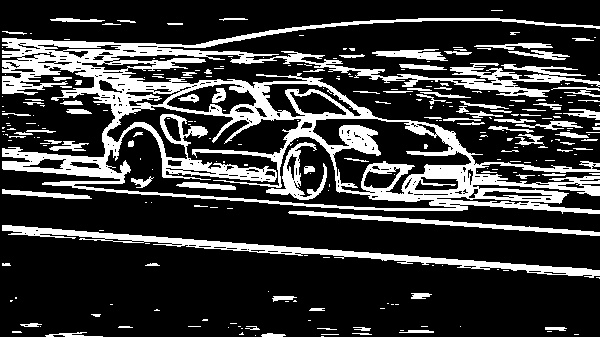
\includegraphics[height=0.15\textwidth, width=0.19\textwidth]{../My_Code/Output/car/car_texture_otsu_RGB.jpg}}
    \subcaptionbox{\large\textbf{e}}{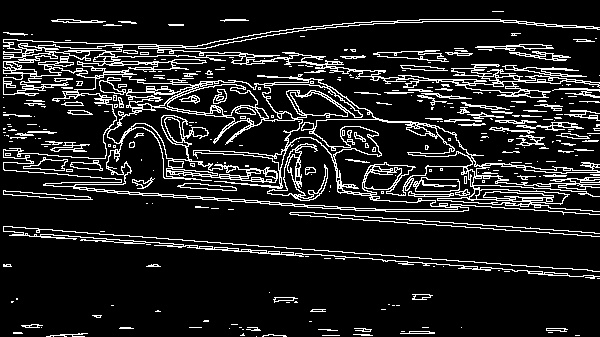
\includegraphics[height=0.15\textwidth, width=0.19\textwidth]{../My_Code/Output/car/car_contour_texture_otsu_RGB.jpg}}
    \caption{Texture-Based Image Segmentation using OTSU Algorithm. Results from channel 1 (a-blue channel), channel 2 (b-green channel) and channel 3 (c-red channel). (d) shows the combined result of all three channels formed by logical AND operation among all masks from all channels.(e) shows the extracted contour from the segmented image.}
    \label{fig:car_3}
\end{figure}

\newpage
\subsection{Image-3}
Foreground = Fox\\
\begin{figure}[!htbp]
     \centering
     \captionsetup[subfigure]{labelformat=empty}
    \subcaptionbox{\large\textbf{a}}{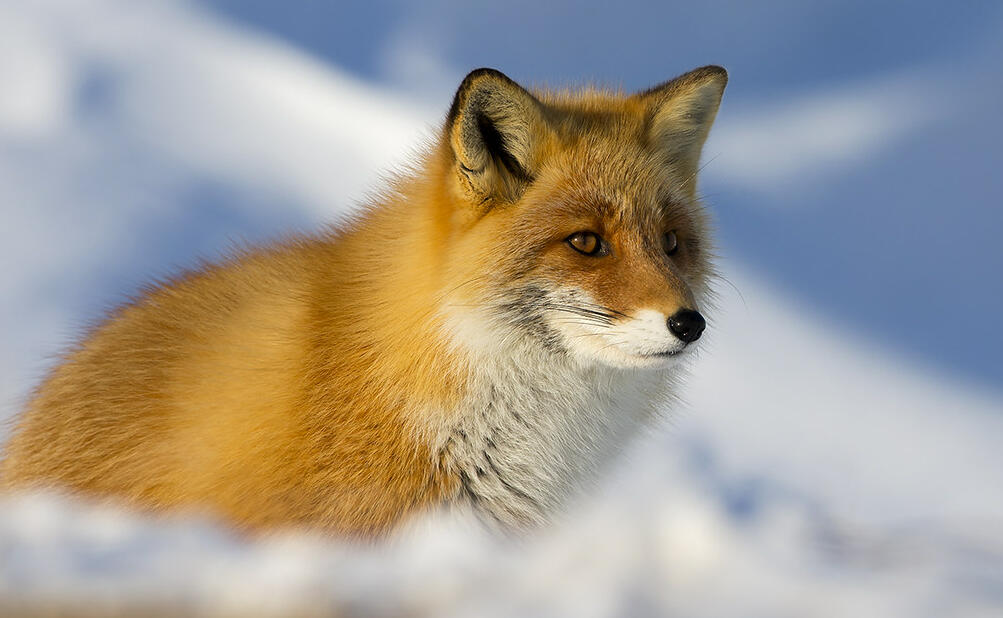
\includegraphics[height=0.15\textwidth, width=0.20\textwidth]{../Images/fox.jpg}}
    \subcaptionbox{\large\textbf{b}}{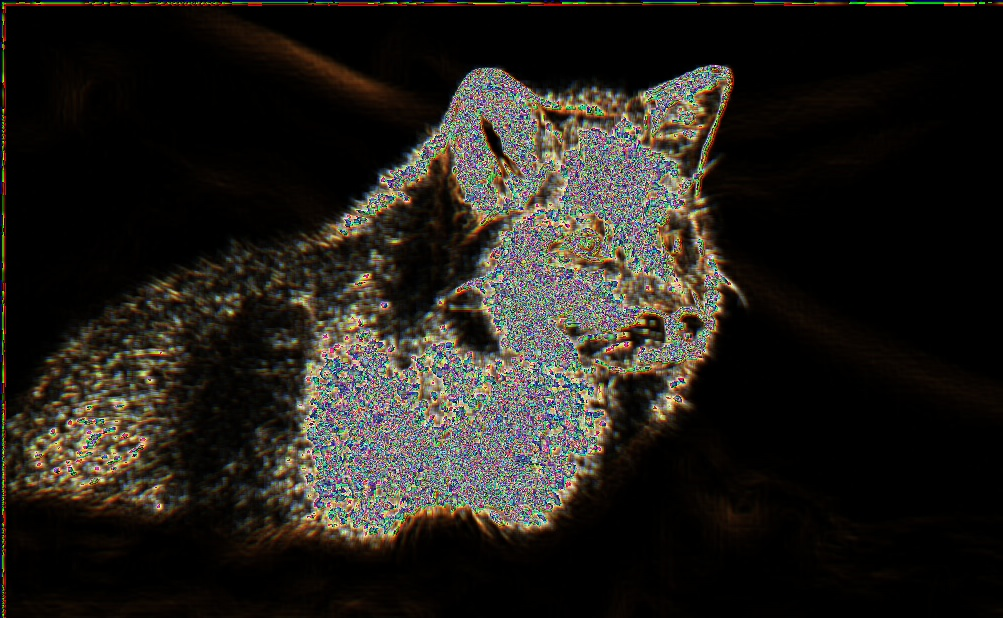
\includegraphics[height=0.15\textwidth, width=0.20\textwidth]{../My_Code/Output/fox/textures_var_fox.jpg}}
    \caption{(a)Input RGB Image. (b)Textured Image formed by $3\times 3$,$5\times 5$ and $7\times 7$ windowed channels.}
    \label{fig:fox_1}
\end{figure}
\begin{figure}[!htbp]
     \centering
    \captionsetup[subfigure]{labelformat=empty}
    \subcaptionbox{\large\textbf{a}}{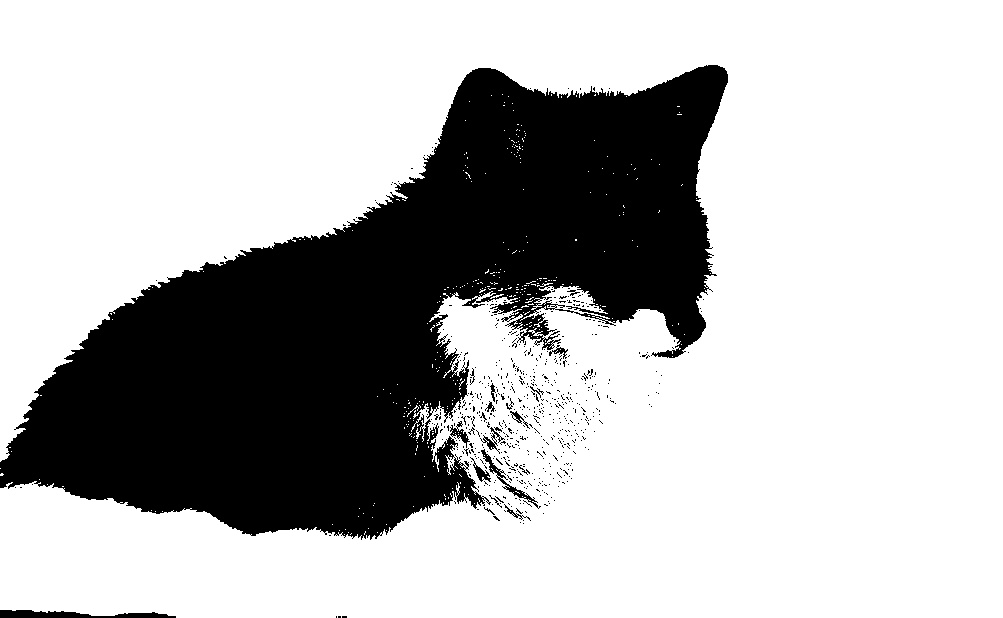
\includegraphics[height=0.15\textwidth, width=0.19\textwidth]{../My_Code/Output/fox/fox_ch_0_otsu_gray_scale.jpg}}
    \subcaptionbox{\large\textbf{b}}{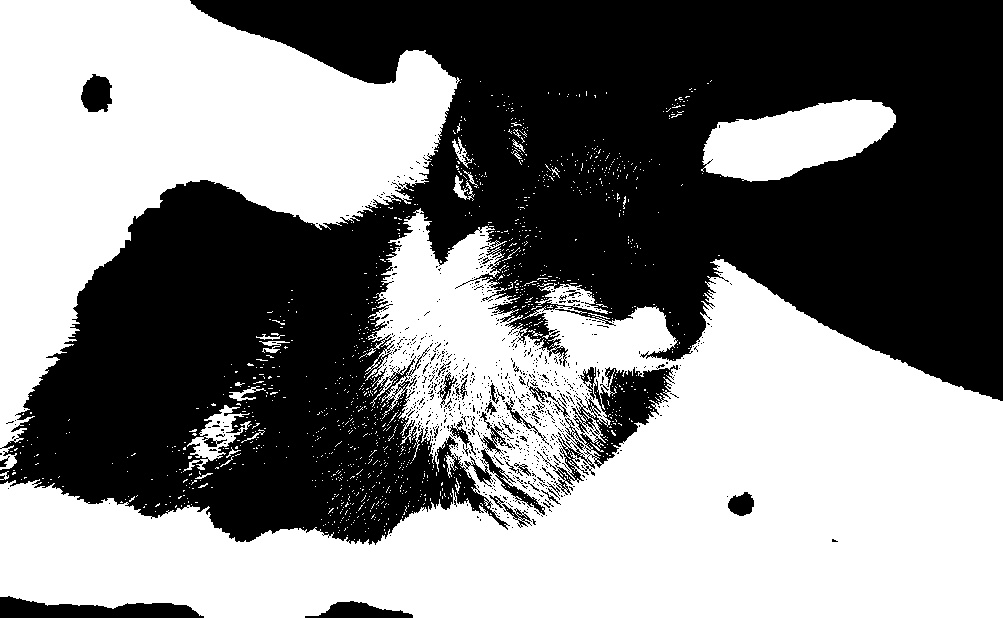
\includegraphics[height=0.15\textwidth, width=0.19\textwidth]{../My_Code/Output/fox/fox_ch_1_otsu_gray_scale.jpg}}
    \subcaptionbox{\large\textbf{c}}{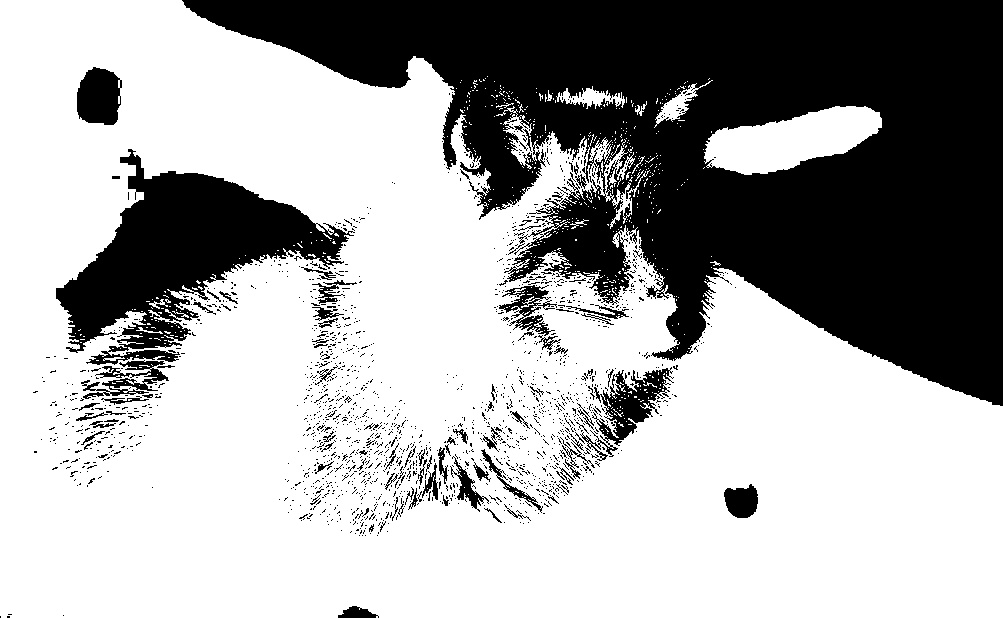
\includegraphics[height=0.15\textwidth, width=0.19\textwidth]{../My_Code/Output/fox/fox_ch_2_otsu_gray_scale.jpg}}
    \subcaptionbox{\large\textbf{d}}{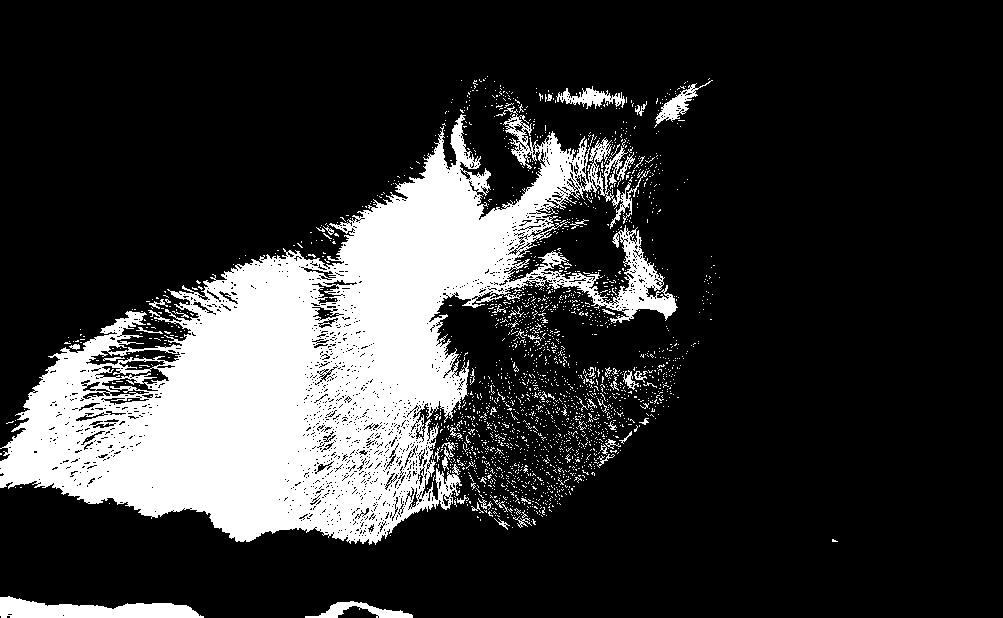
\includegraphics[height=0.15\textwidth, width=0.19\textwidth]{../My_Code/Output/fox/fox_otsu_RGB.jpg}}
    \subcaptionbox{\large\textbf{e}}{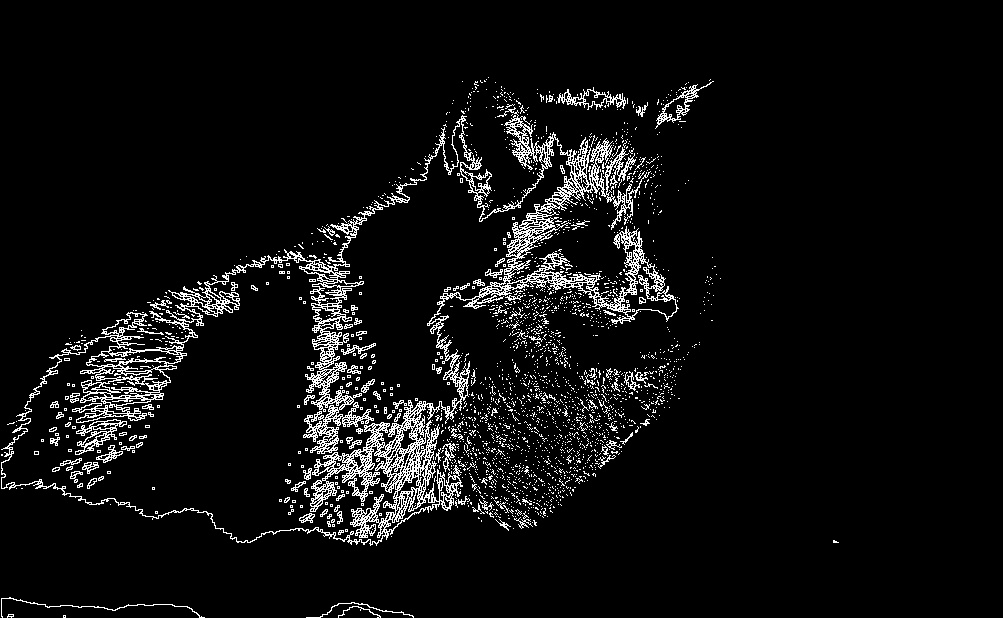
\includegraphics[height=0.15\textwidth, width=0.19\textwidth]{../My_Code/Output/fox/fox_contour_raw_otsu_RGB.jpg}}
    \caption{RGB-Based Image Segmentation using OTSU Algorithm. Results from channel 1 (a-blue channel), channel 2 (b-green channel) and channel 3 (c-red channel). (d) shows the combined result of all three channels by the operation [AND(R,R-AND(G,B))]. Here, R,G,B are three different channels. (e) shows the extracted contour from the segmented image.}
    \label{fig:fox_2}
\end{figure}
\begin{figure}[!htbp]
     \centering
    \captionsetup[subfigure]{labelformat=empty}
    \subcaptionbox{\large\textbf{a}}{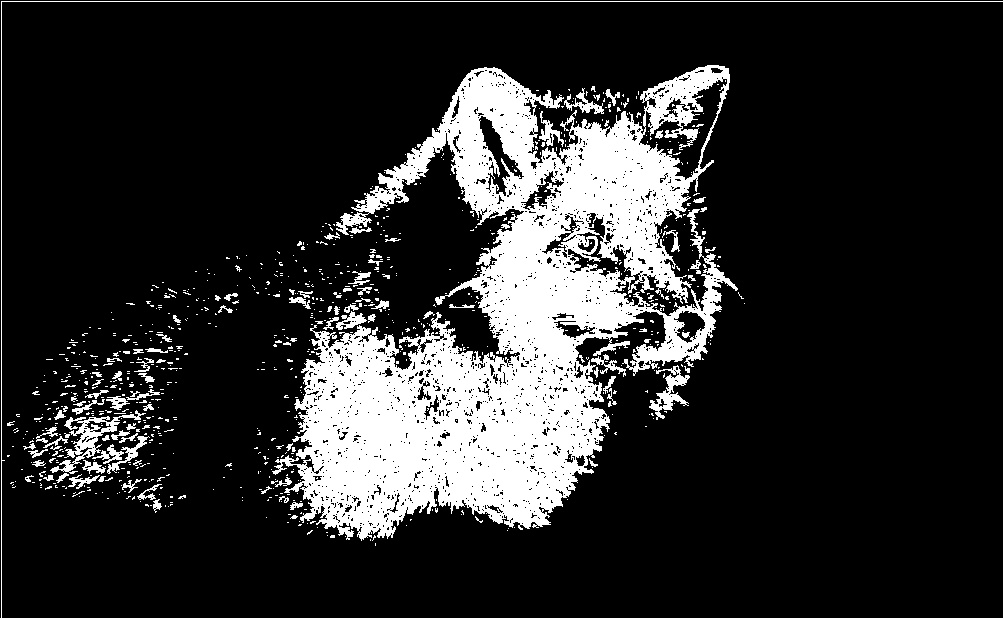
\includegraphics[height=0.15\textwidth, width=0.19\textwidth]{../My_Code/Output/fox/fox_texture_ch_0_otsu_gray_scale.jpg}}
    \subcaptionbox{\large\textbf{b}}{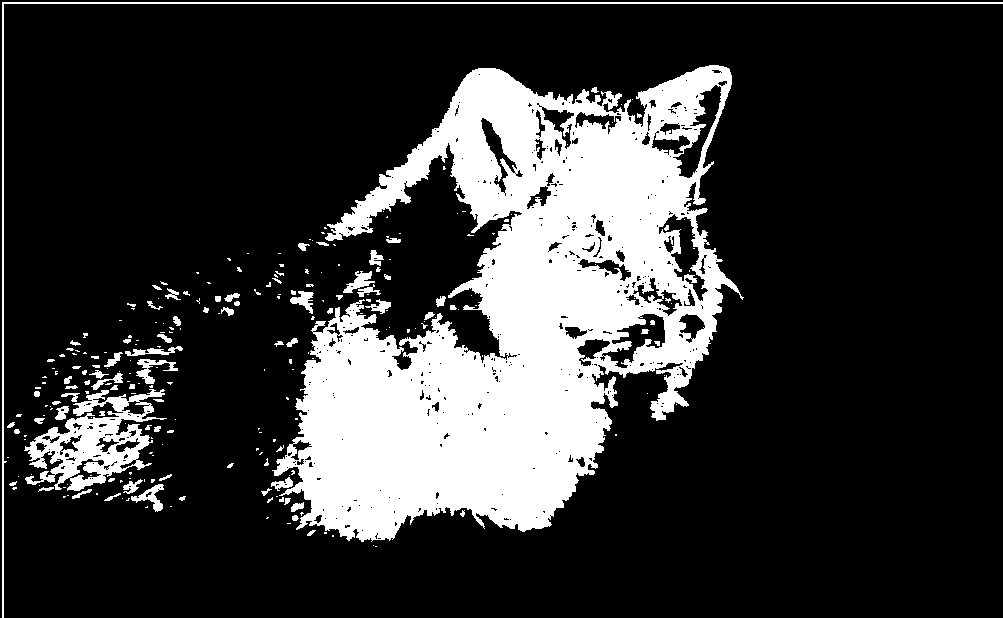
\includegraphics[height=0.15\textwidth, width=0.19\textwidth]{../My_Code/Output/fox/fox_texture_ch_1_otsu_gray_scale.jpg}}
    \subcaptionbox{\large\textbf{c}}{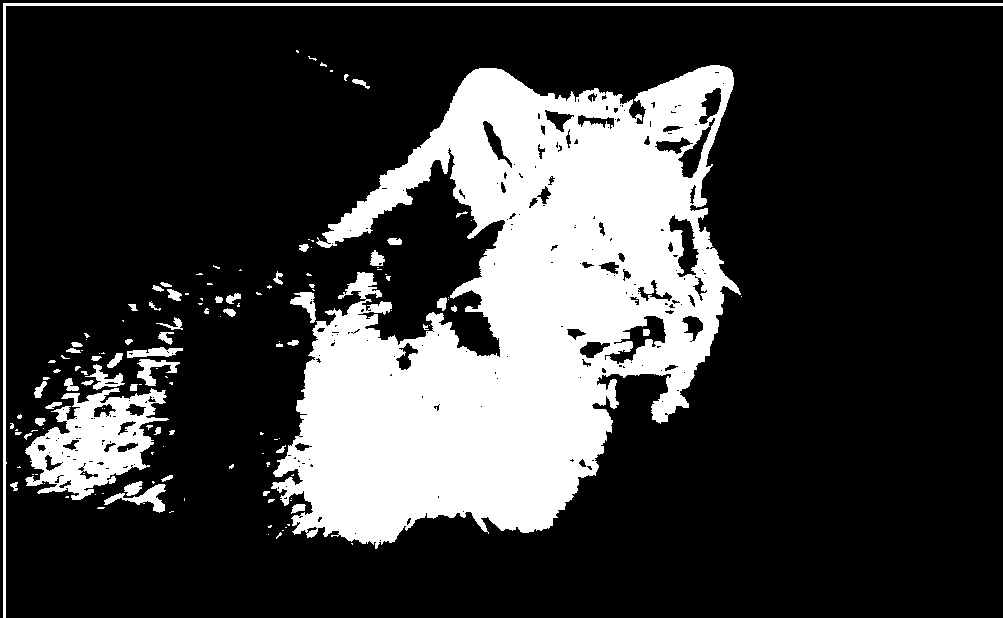
\includegraphics[height=0.15\textwidth, width=0.19\textwidth]{../My_Code/Output/fox/fox_texture_ch_2_otsu_gray_scale.jpg}}
    \subcaptionbox{\large\textbf{d}}{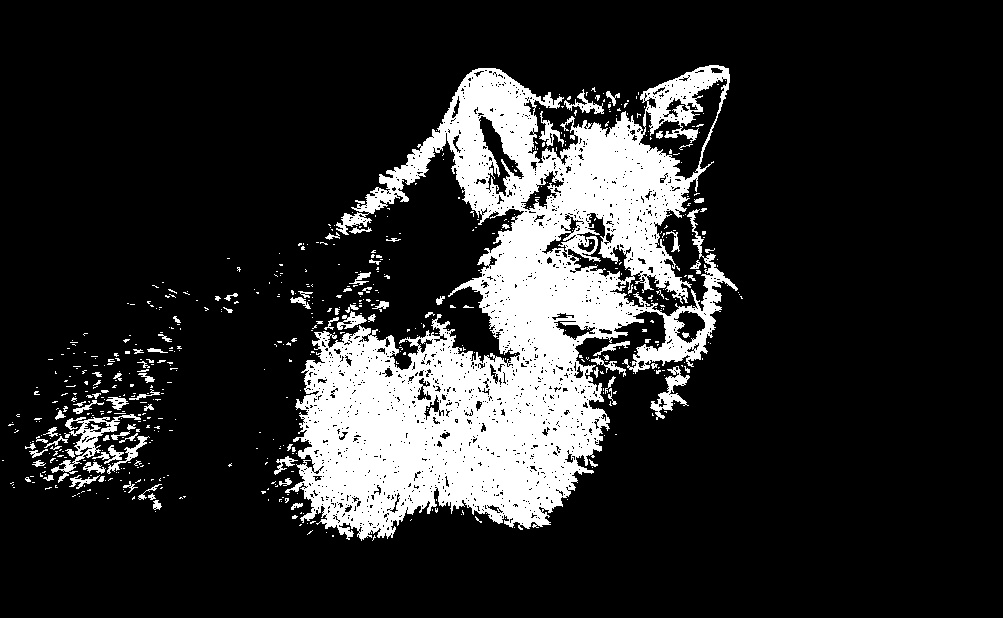
\includegraphics[height=0.15\textwidth, width=0.19\textwidth]{../My_Code/Output/fox/fox_texture_otsu_RGB.jpg}}
    \subcaptionbox{\large\textbf{e}}{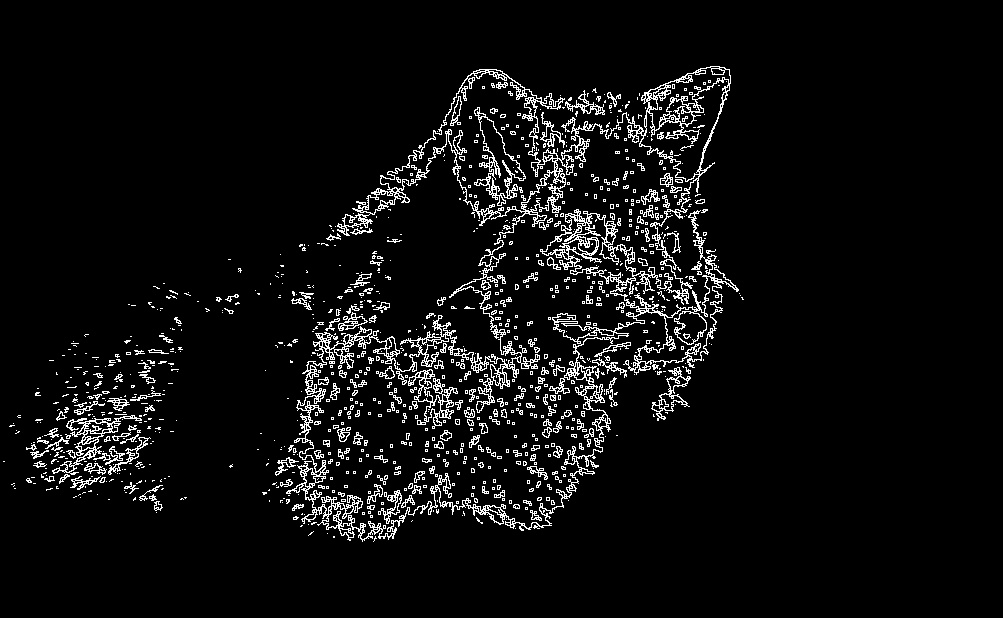
\includegraphics[height=0.15\textwidth, width=0.19\textwidth]{../My_Code/Output/fox/fox_contour_texture_otsu_RGB.jpg}}
    \caption{Texture-Based Image Segmentation using OTSU Algorithm. Results from channel 1 (a-blue channel), channel 2 (b-green channel) and channel 3 (c-red channel). (d) shows the combined result of all three channels formed by logical AND operation among all masks from all channels.(e) shows the extracted contour from the segmented image.}
    \label{fig:fox_3}
\end{figure}

\newpage
\subsection{Image-4}
Foreground = Lady with Fox\\
\begin{figure}[!htbp]
     \centering
     \captionsetup[subfigure]{labelformat=empty}
    \subcaptionbox{\large\textbf{a}}{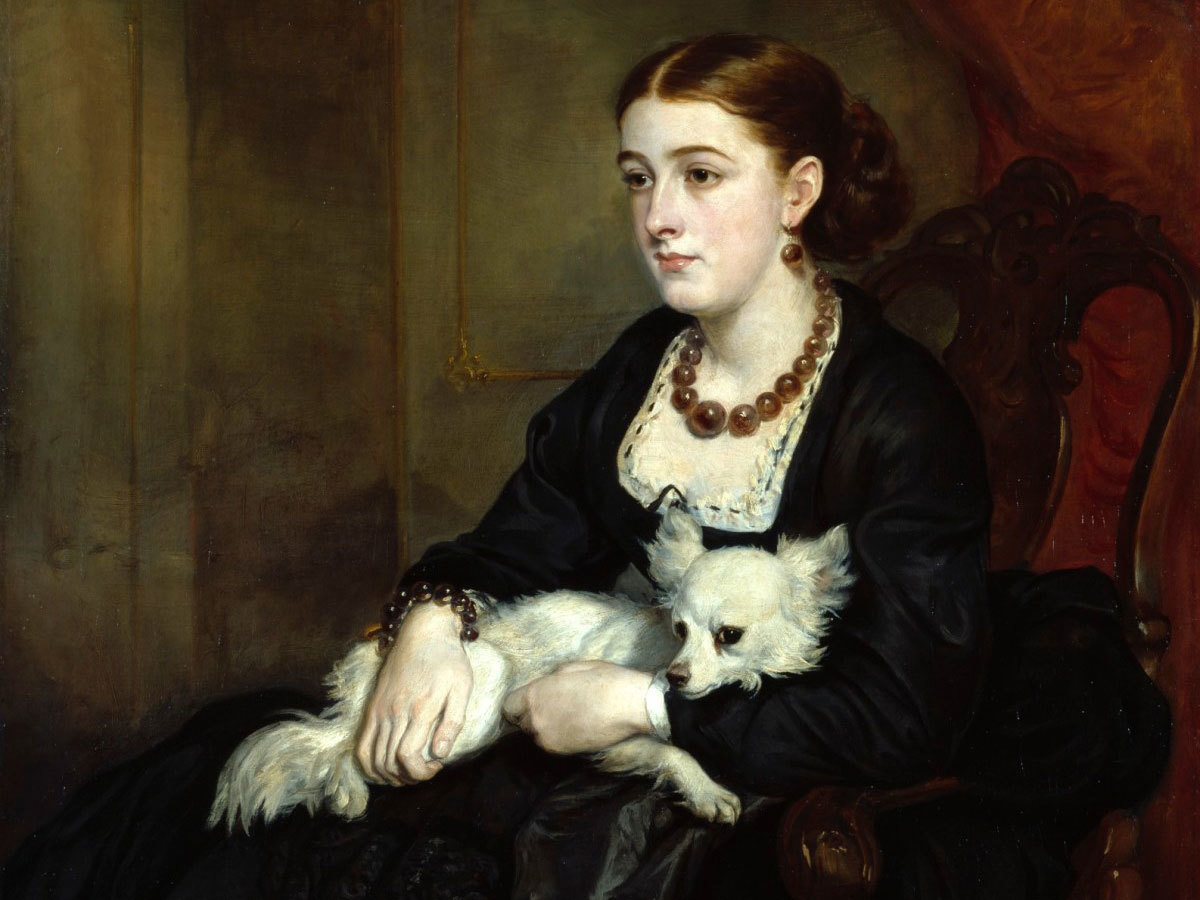
\includegraphics[width=0.20\textwidth]{../Images/portrait.jpg}}
    \subcaptionbox{\large\textbf{b}}{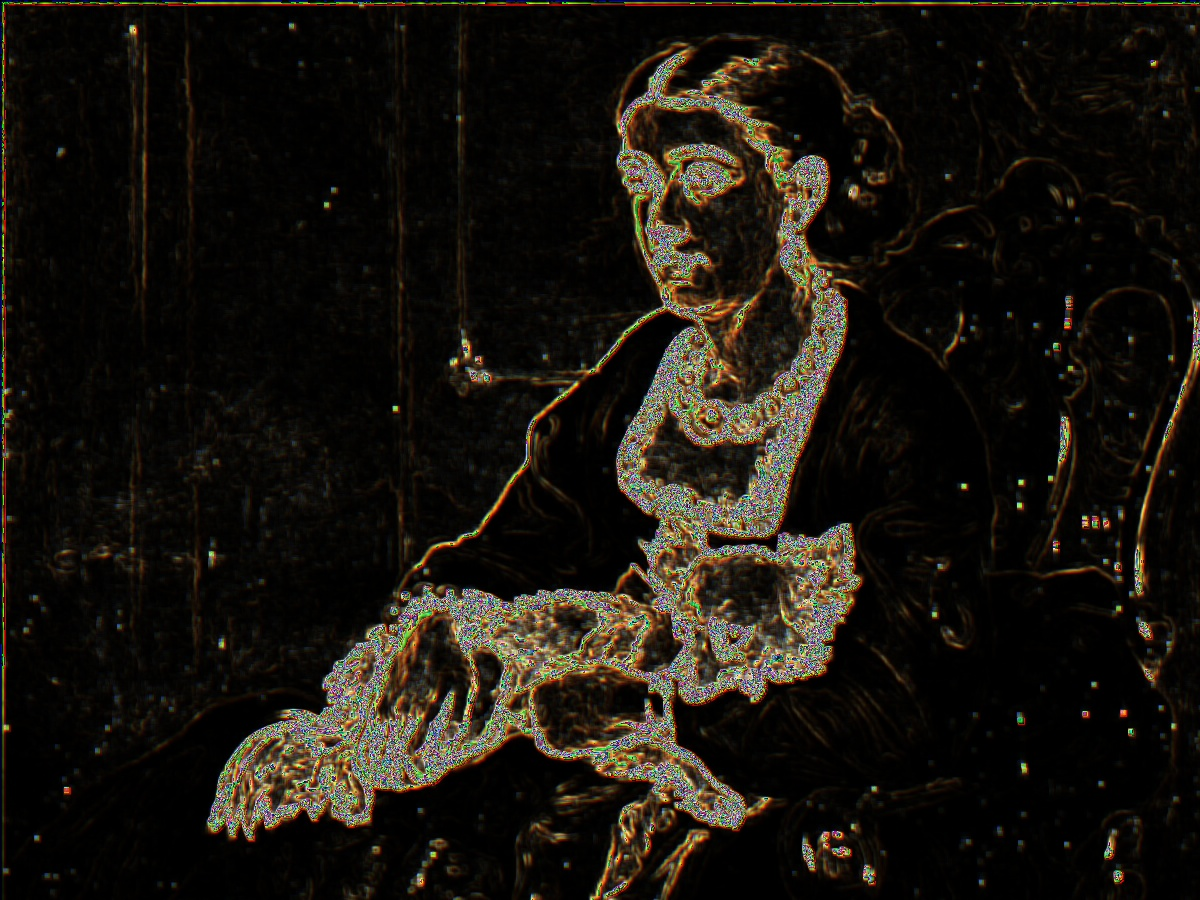
\includegraphics[width=0.20\textwidth]{../My_Code/Output/portrait/textures_var_portrait.jpg}}
    \caption{(a)Input RGB Image. (b)Textured Image formed by $3\times 3$,$5\times 5$ and $7\times 7$ windowed channels.}
\end{figure}
\begin{figure}[!htbp]
     \centering
    \captionsetup[subfigure]{labelformat=empty}
    \subcaptionbox{\large\textbf{a}}{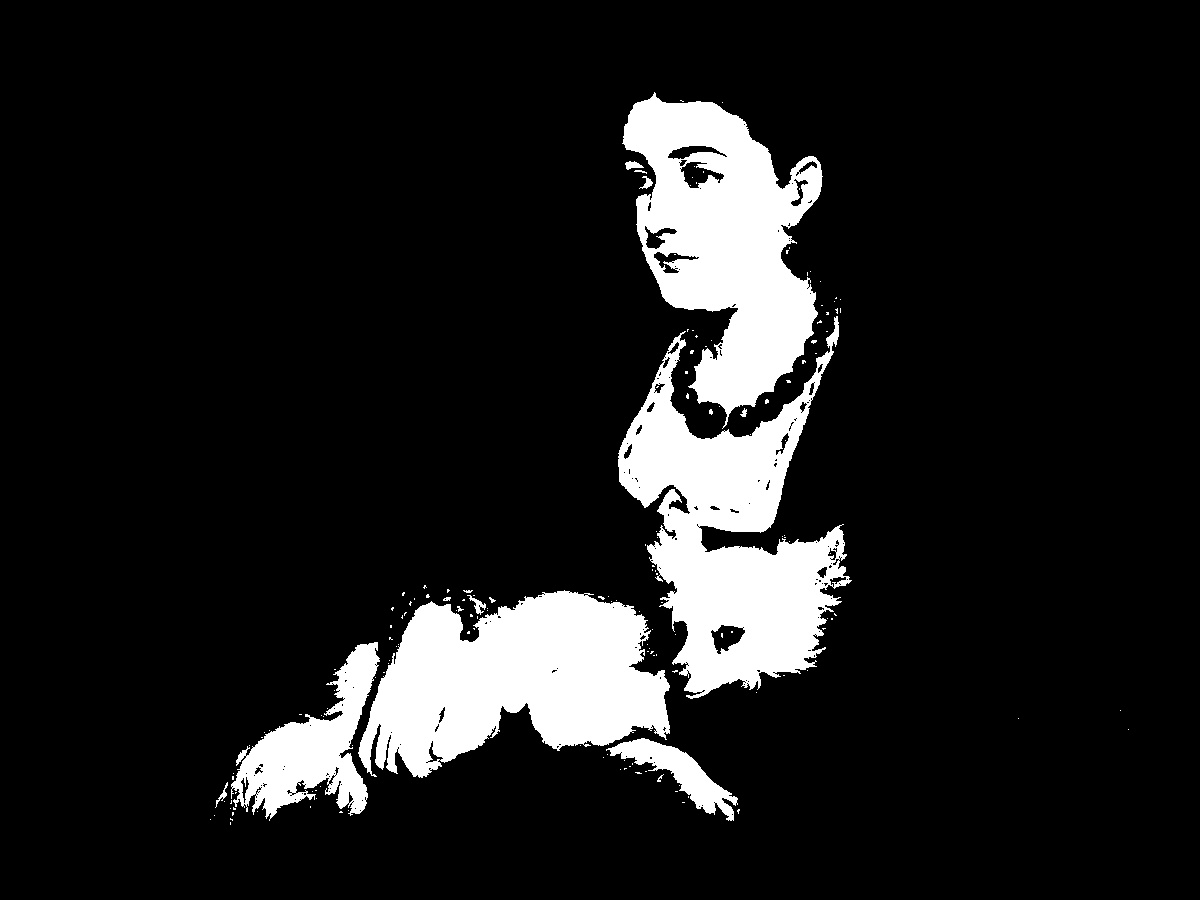
\includegraphics[width=0.19\textwidth]{../My_Code/Output/portrait/portrait_ch_0_otsu_gray_scale.jpg}}
    \subcaptionbox{\large\textbf{b}}{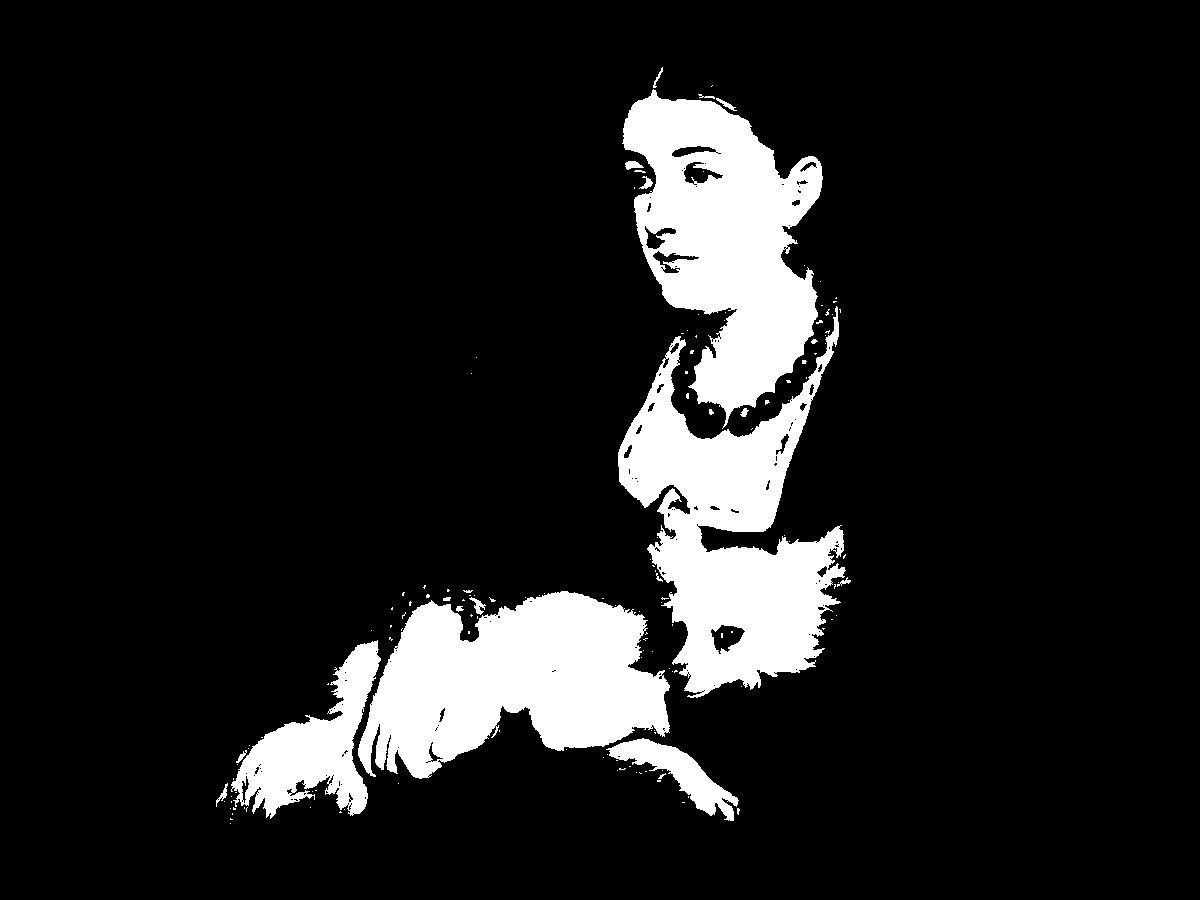
\includegraphics[width=0.19\textwidth]{../My_Code/Output/portrait/portrait_ch_1_otsu_gray_scale.jpg}}
    \subcaptionbox{\large\textbf{c}}{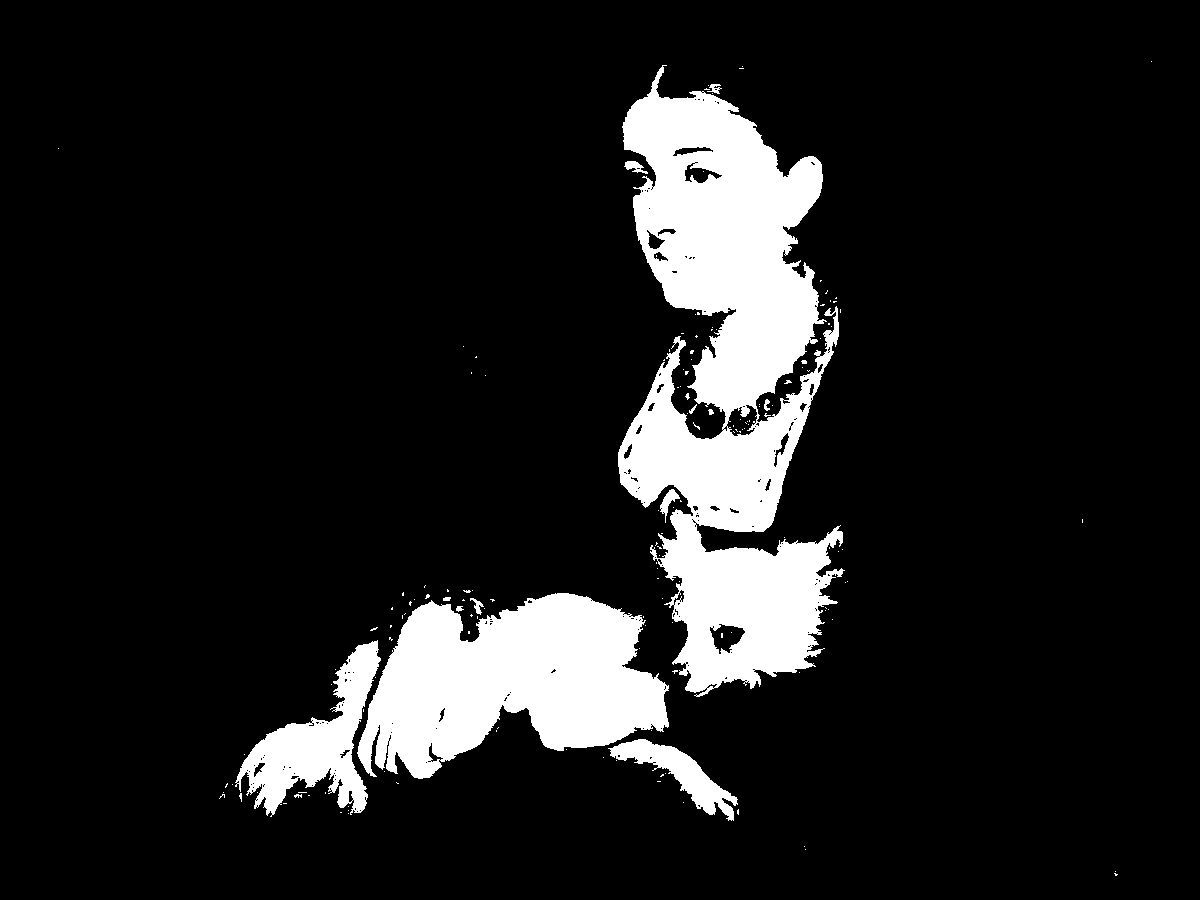
\includegraphics[width=0.19\textwidth]{../My_Code/Output/portrait/portrait_ch_2_otsu_gray_scale.jpg}}
    \subcaptionbox{\large\textbf{d}}{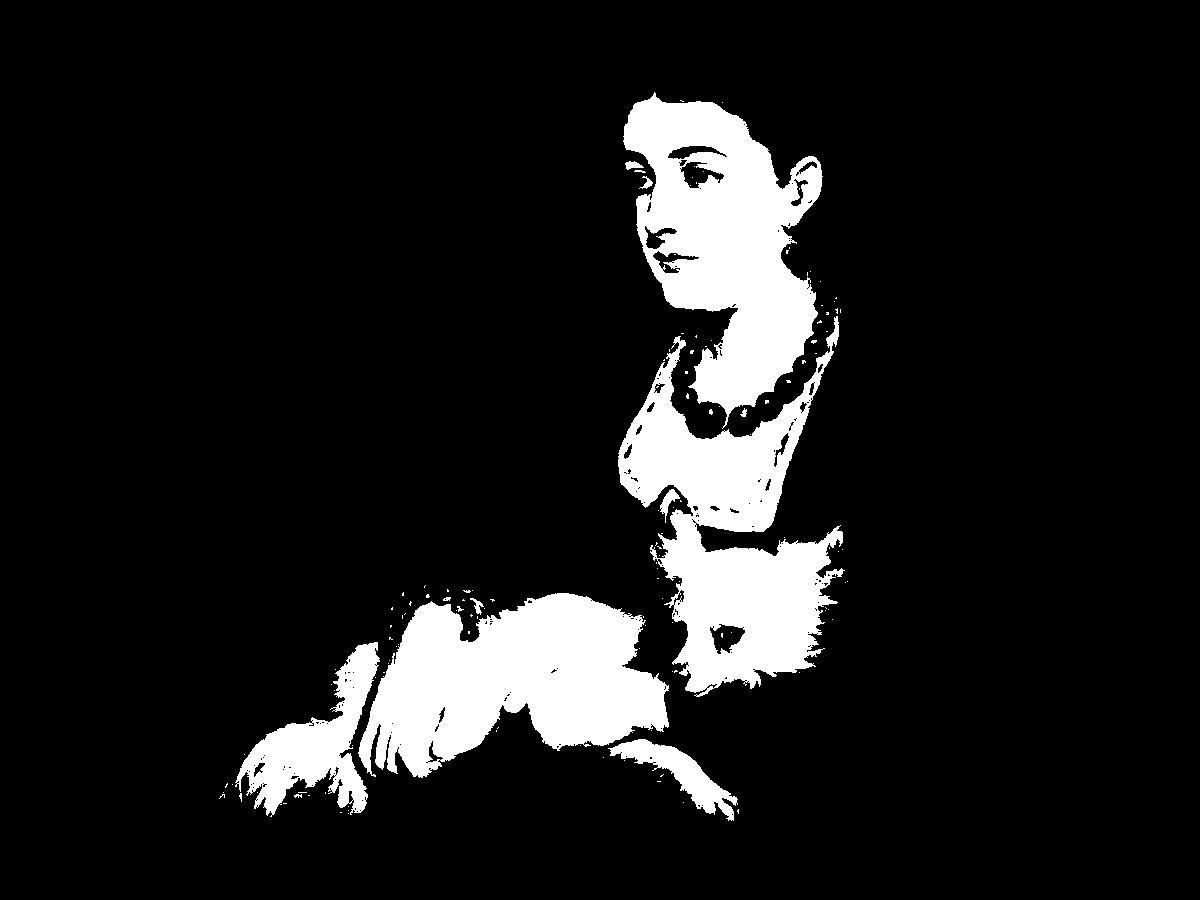
\includegraphics[width=0.19\textwidth]{../My_Code/Output/portrait/portrait_otsu_RGB.jpg}}
    \subcaptionbox{\large\textbf{e}}{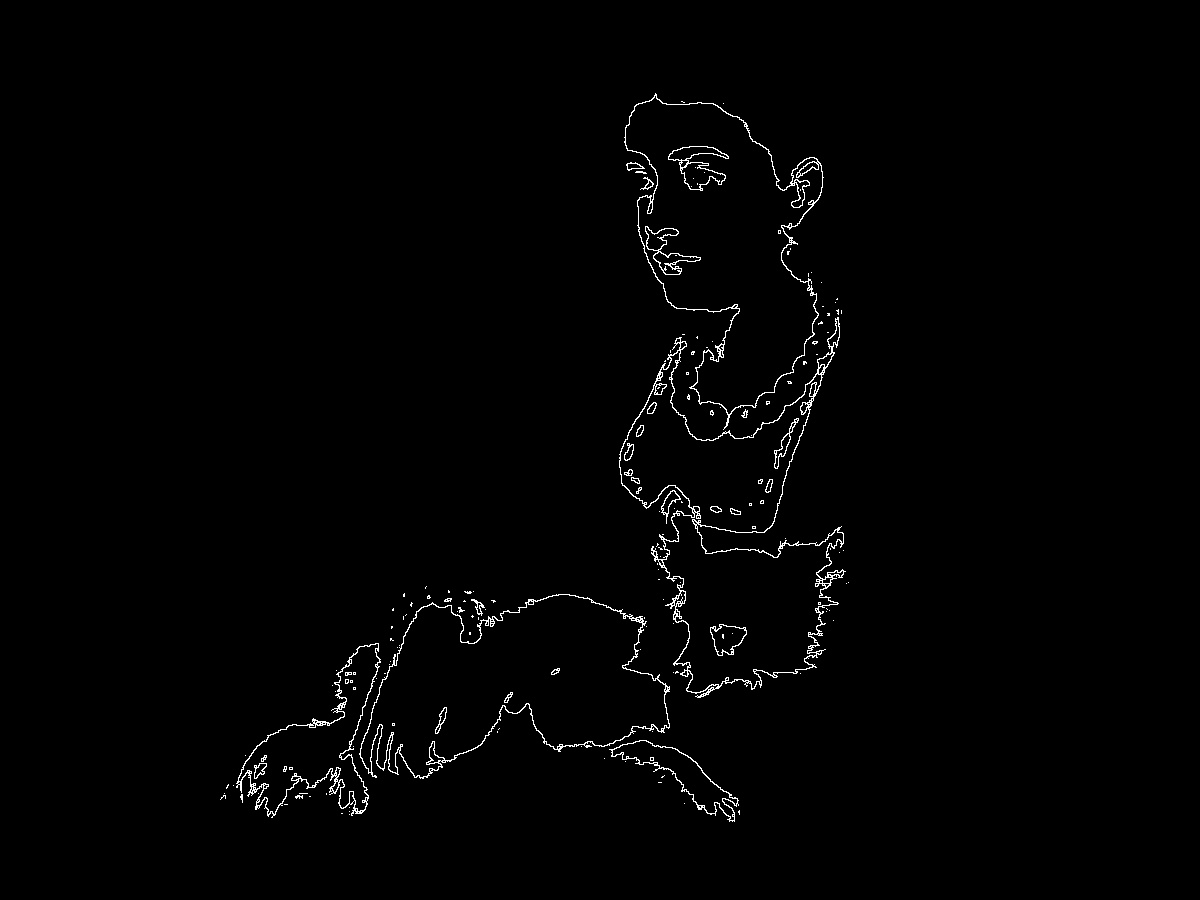
\includegraphics[width=0.19\textwidth]{../My_Code/Output/portrait/portrait_contour_raw_otsu_RGB.jpg}}
    \caption{RGB-Based Image Segmentation using OTSU Algorithm. Results from channel 1 (a-blue channel), channel 2 (b-green channel) and channel 3 (c-red channel). (d) shows the combined result of all three channels formed by logical AND operation among all masks from all channels.(e) shows the extracted contour from the segmented image.}
\end{figure}
\begin{figure}[!htbp]
     \centering
    \captionsetup[subfigure]{labelformat=empty}
    \subcaptionbox{\large\textbf{a}}{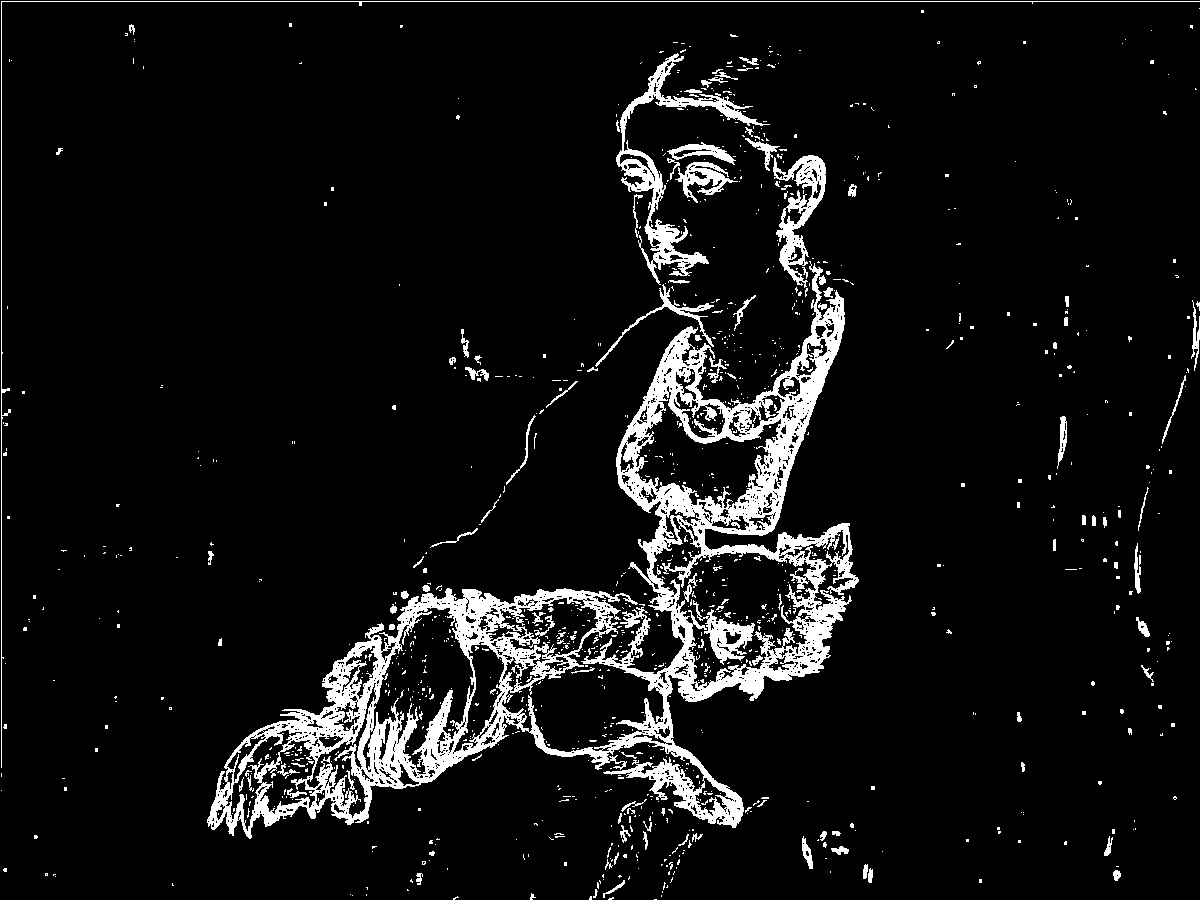
\includegraphics[width=0.19\textwidth]{../My_Code/Output/portrait/portrait_texture_ch_0_otsu_gray_scale.jpg}}
    \subcaptionbox{\large\textbf{b}}{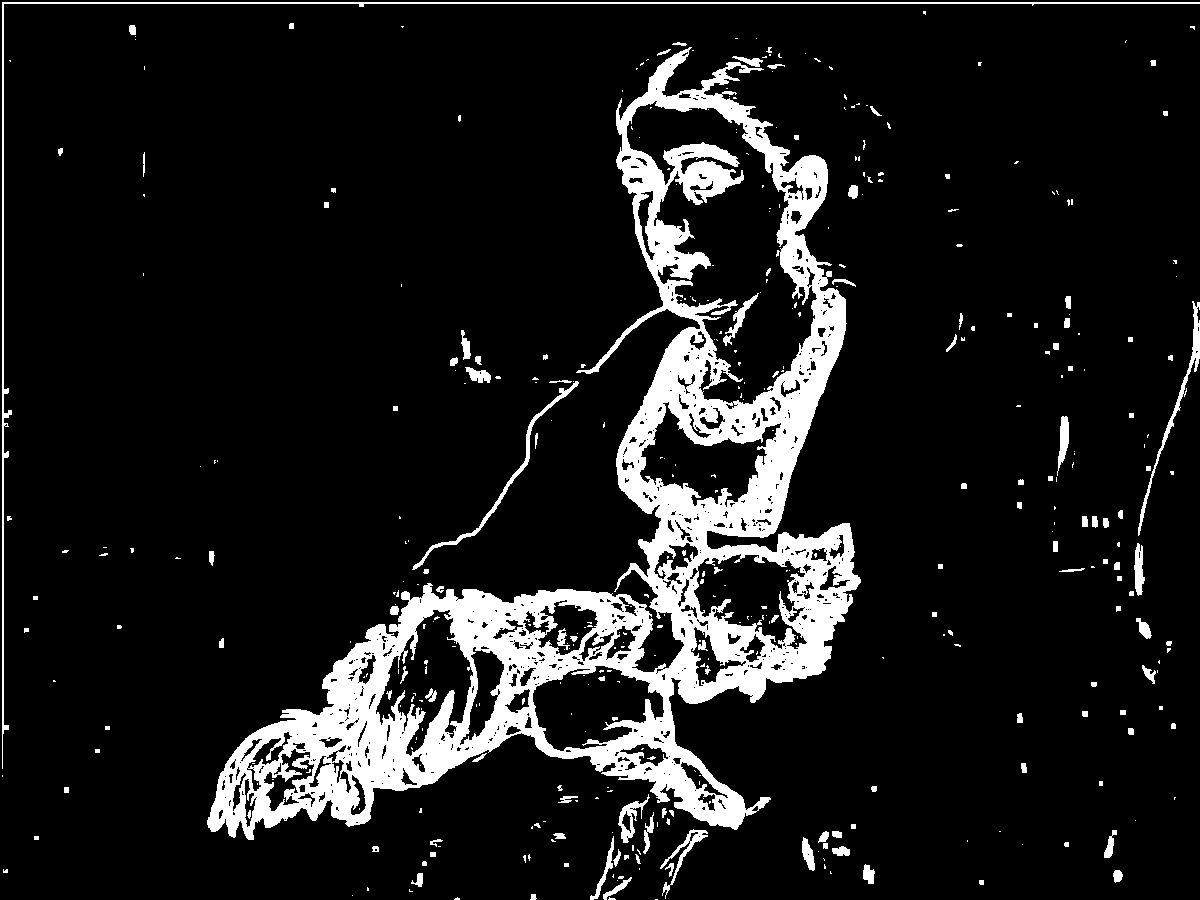
\includegraphics[width=0.19\textwidth]{../My_Code/Output/portrait/portrait_texture_ch_1_otsu_gray_scale.jpg}}
    \subcaptionbox{\large\textbf{c}}{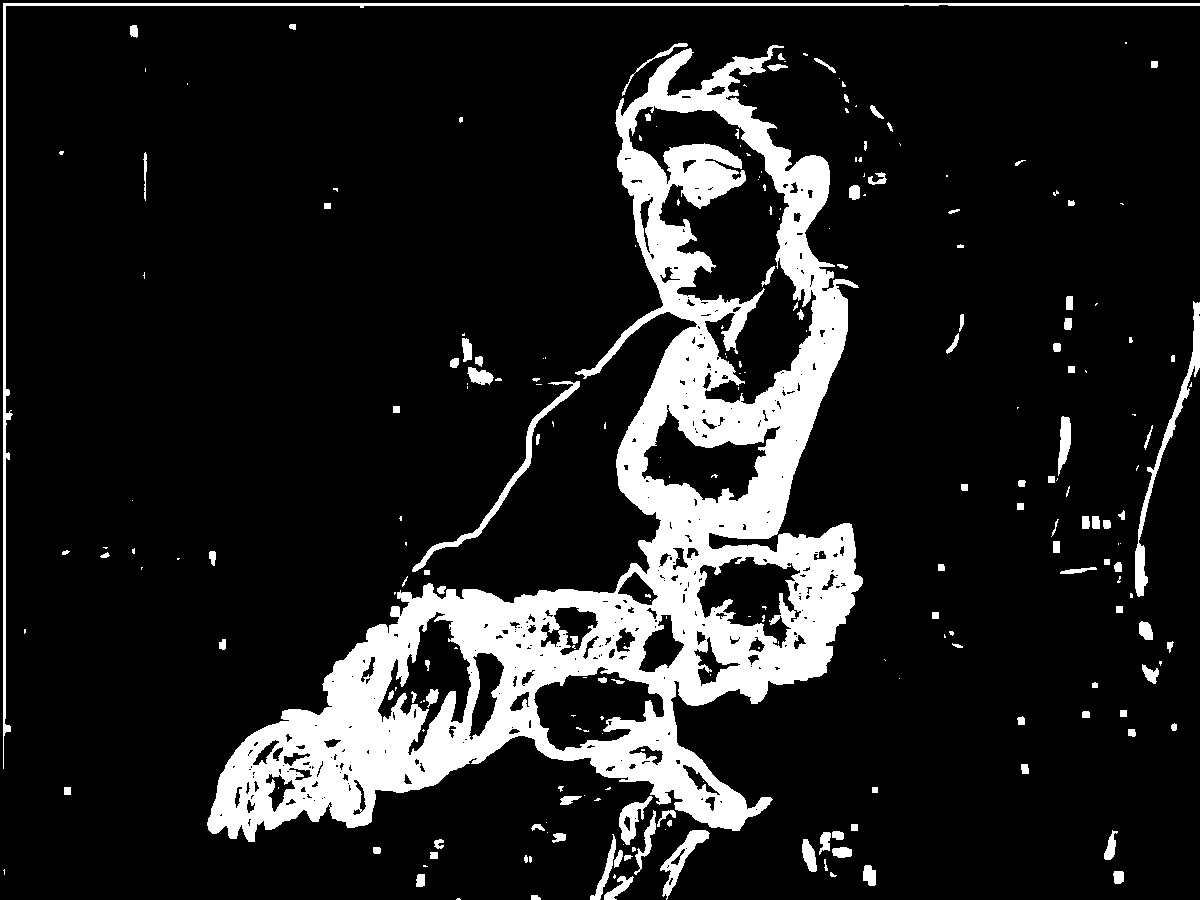
\includegraphics[width=0.19\textwidth]{../My_Code/Output/portrait/portrait_texture_ch_2_otsu_gray_scale.jpg}}
    \subcaptionbox{\large\textbf{d}}{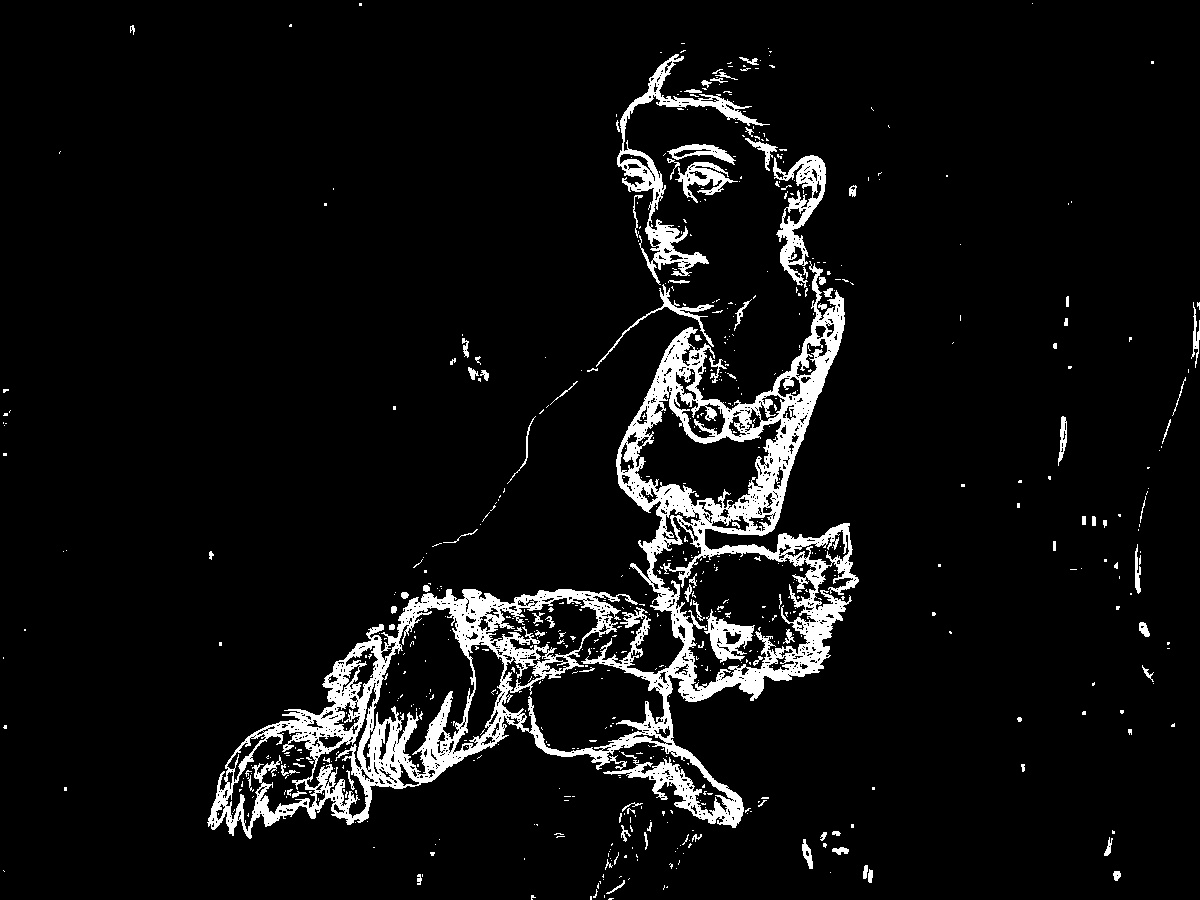
\includegraphics[width=0.19\textwidth]{../My_Code/Output/portrait/portrait_texture_otsu_RGB.jpg}}
    \subcaptionbox{\large\textbf{e}}{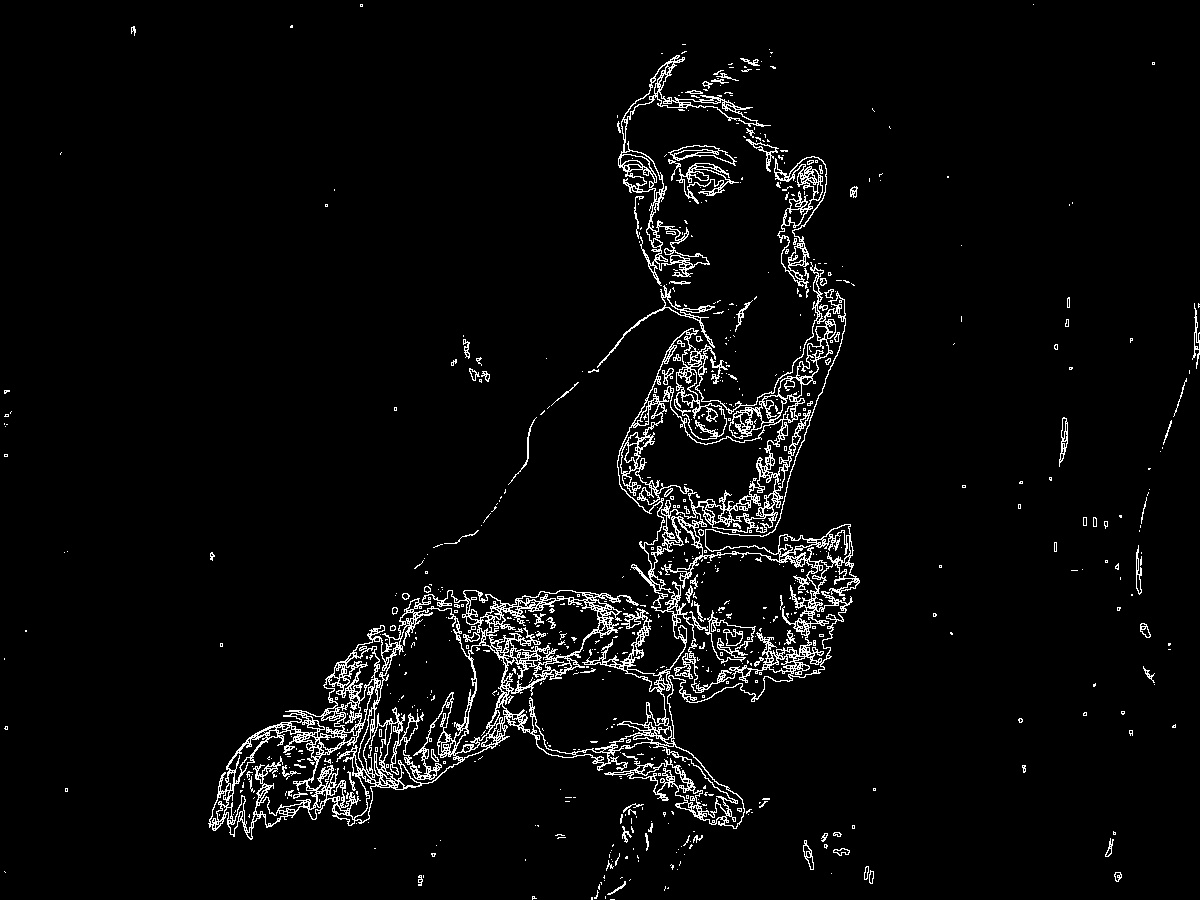
\includegraphics[width=0.19\textwidth]{../My_Code/Output/portrait/portrait_contour_texture_otsu_RGB.jpg}}
    \caption{Texture-Based Image Segmentation using OTSU Algorithm. Results from channel 1 (a-blue channel), channel 2 (b-green channel) and channel 3 (c-red channel). (d) shows the combined result of all three channels formed by logical AND operation among all masks from all channels.(e) shows the extracted contour from the segmented image.}
    \label{fig:painting}
\end{figure}

\newpage
\section{Discussion}
\begin{itemize}
\item It seems the results are highly dependent on the input image and its color channels.
\item For some images, most of the rlevent feature informations are inside a single channel. In those cases, simple Logical AND operation among the mask of different channels from OTSU algorithm will not provide a good result. For example. look in the RGB based segmentation results of cat, car and fox image. Fo the case of cat (Fig. \ref{fig:cat_1}) and fox(Fig. \ref{fig:fox_1}), red channel is highest priority, but for the car green channel is of highest priority. Hence, we did a special combination of these channels based on the following formaula-
\begin{equation}
	Mask = AND(Mask_R, (Mask_R - OR(Mask_{IR}))
\end{equation}
Here, $Mask_R$ denotes the mask from the most relevant channel. $Mask_{IR}$ denotes the irrelevant channels. 'AND' and 'OR' signify the logical 'and' and 'or' operation, respectively. This modification provides a better segmentation result.
\item The RGB based segmentation method seems to provide considerably good results with some modifications as stated in the previous point. However, sometimes, this methodgets erroneos results when the foreground object is overlapping with some other objects as evident from the cat (Fig. \ref{fig:cat_2}) and car (Fig. \ref{fig:car_2}) image.
\item Texture feature based segmentation method is more susceptible to noise than the RGB base segmentation method. It is best shown in the painting image in Fig. \ref{fig:painting}. However, if the foreground features are must prominent than the background (such as the fox image in Fig. \ref{fig:fox_1} and Fig. \ref{fig:fox_3}, the image is taken by blurring the background, i.e. in portrait mode of digital cameras), the texture-feature based segmentation can provide considerably good results. On the other hand, if all channels of the image contain relevant features with equal probability, the method will not provide good segmentation (as evident from Fig. \ref{fig:car_3}).
\end{itemize}

\newpage
\section{Source Code}
\begin{lstlisting}[language=Python]
import cv2, os
import numpy as np
import math
from scipy.stats import entropy

def image_read(fname, gray_scale=False):
	if gray_scale:
		im = cv2.imread(fname,cv2.IMREAD_GRAYSCALE)
	else:
		im = cv2.imread(fname)
	return im
def image_texture(image,N,feature,out_dir,name):
	#N = window size = N*N
	save_dir = out_dir+'/'+name
	if not os.path.exists(save_dir):
		os.makedirs(save_dir)
	gray_image = image
	if len(list(gray_image.shape))>2:
		gray_image = cv2.cvtColor(gray_image,cv2.COLOR_BGR2GRAY)
	textures = np.zeros((image.shape[0],image.shape[1],len(N)))

	for tx in range(0,len(N)):
		padding = int(N[tx]/2)
		padded_image = np.pad(gray_image,((padding,padding),(padding,padding)),mode='constant',constant_values=0)
		if feature.upper() == 'VAR':
			for ix in range(padding,padded_image.shape[0]-2*padding):
				for jx in range(padding,padded_image.shape[1]-2*padding):
					textures[ix,jx,tx] = np.var(padded_image[ix-padding:ix+padding+1,jx-padding:jx+padding+1])
		elif feature.upper() == "ENTROPY":
			for ix in range(padding,padded_image.shape[0]-2*padding):
				for jx in range(padding,padded_image.shape[1]-2*padding):
					val,cnt = np.unique(padded_image[ix-padding:ix+padding+1,jx-padding:jx+padding+1], return_counts=True)
					norm_cnt = cnt / cnt.sum()
					textures[ix,jx,tx] = -(norm_cnt * np.log(norm_cnt)/np.log(math.e)).sum()
		else:
			print("Please provide a valid feature name")
	cv2.imwrite(save_dir+"/textures_"+feature+"_"+name+".jpg",textures.astype(np.uint8))
	return textures
def otsu_gray_scale(epochs,image,out_dir,name):
	save_dir = out_dir+'/'+name.split("_")[0]
	if not os.path.exists(save_dir):
		os.makedirs(save_dir)
	N = np.prod(image.shape)#Total number of pixels in the image
	mask = np.ones(image.shape)
	for ix in range(0,epochs):
		image_new = np.multiply(image,mask)
		sigma_optimum = 0
		k_optimum = 0
		hist,bin_edges = np.histogram(image_new,bins=np.arange(256))
		p = hist/N#probability of each bin
		for k in range(0,256):
			#k = grayscale threshold level
			w0 = np.sum(p[:k])
			w1 = np.sum(p[k:])
			P = np.multiply(p,np.arange(1,256,1))
			if w0>0 and w1>0:
				mu0 = np.sum(P[:k])/w0
				mu1 = np.sum(P[k:])/w1
				sigma = w0*w1*(mu0-mu1)**2
				if sigma>=sigma_optimum:
					sigma_optimum=sigma
					k_optimum=k
		mask = np.where(image_new<k_optimum,0,1)
		image = image_new
		print("Epoch = ",str(ix),' k_optimum = ',str(k_optimum),' sigma_optimum = ',str(sigma_optimum))
	cv2.imwrite(save_dir+'/'+name+'_otsu_gray_scale.jpg',(mask*255).astype(np.uint8))
	return mask,sigma_optimum,k_optimum
def otsu_RGB(epochs,image,out_dir,name,special_case=False):
	save_dir = out_dir+'/'+name.split("_")[0]
	if not os.path.exists(save_dir):
		os.makedirs(save_dir)
	nb_channels = image.shape[-1]
	final_mask = []
	for ch in range(0,nb_channels):
		print('\n\nChannel = ',ch)
		mask,_,_ = otsu_gray_scale(epochs,image[:,:,ch],out_dir,name+'_ch_'+str(ch))
		final_mask.append(mask)
	if special_case:
		if name in ['cat','fox']:
			final_mask = np.logical_and(final_mask[2],final_mask[2]-np.logical_and(final_mask[0],final_mask[1]))
		elif name in ['car']:
			final_mask = np.logical_and(final_mask[1],final_mask[1]-np.logical_and(final_mask[2],final_mask[0]))
	else:
		final_mask = np.logical_and(final_mask[0],final_mask[1],final_mask[2])
	cv2.imwrite(save_dir+'/'+name+'_otsu_RGB.jpg',(final_mask*255).astype(np.uint8))
	return final_mask
def find_contour(mask,out_dir,name,reverse_contour=False):
	save_dir = out_dir+'/'+name.split("_")[0]
	if not os.path.exists(save_dir):
		os.makedirs(save_dir)
	contour = np.zeros(mask.shape)
	padding=1
	mask = np.pad(mask,((padding,padding),(padding,padding)),mode='constant',constant_values=0)
	for ix in range(padding,mask.shape[0]-2*padding):
		for jx in range(padding,mask.shape[1]-2*padding):
			if mask[ix,jx] == 1:
				if 0 in mask[ix-padding:ix+padding+1,jx-padding:jx+padding+1]:
					contour[ix,jx] = 1

	if reverse_contour:
		contour = np.abs(-1+contour)
	cv2.imwrite(save_dir+'/'+name+'_otsu_RGB.jpg',(contour*255).astype(np.uint8))
	return contour

def Main():
	out_dir = './Output'

	image_name = "cat"
	fname = "../Images/"+image_name+".jpg"
	I1 = image_read(fname)
	mask_from_raw = otsu_RGB(10,I1,out_dir,image_name,special_case=True)
	contour = find_contour(mask_from_raw,out_dir,image_name+'_contour_raw')
	features = 'var'#options = "var","entropy"
	N = [3,5,7]
	textures = image_texture(I1,N,features,out_dir,image_name)
	mask_from_texture = otsu_RGB(10,textures,out_dir,image_name+'_texture')
	contour = find_contour(mask_from_texture,out_dir,image_name+'_contour_texture')


	image_name = "car"
	fname = "../Images/"+image_name+".jpg"
	I1 = image_read(fname)
	mask_from_raw = otsu_RGB(10,I1,out_dir,image_name,special_case=True)
	contour = find_contour(mask_from_raw,out_dir,image_name+'_contour_raw')
	features = 'var'#options = "var","entropy"
	N = [3,4,5]
	textures = image_texture(I1,N,features,out_dir,image_name)
	mask_from_texture = otsu_RGB(10,textures,out_dir,image_name+'_texture')
	contour = find_contour(mask_from_texture,out_dir,image_name+'_contour_texture')


	image_name = "fox"
	fname = "../Images/"+image_name+".jpg"
	I1 = image_read(fname)
	mask_from_raw = otsu_RGB(10,I1,out_dir,image_name,special_case=True)
	contour = find_contour(mask_from_raw,out_dir,image_name+'_contour_raw')
	features = 'var'#options = "var","entropy"
	N = [3,5,7]
	textures = image_texture(I1,N,features,out_dir,image_name)
	mask_from_texture = otsu_RGB(10,textures,out_dir,image_name+'_texture')
	contour = find_contour(mask_from_texture,out_dir,image_name+'_contour_texture')


	image_name = "portrait"
	fname = "../Images/"+image_name+".jpg"
	I1 = image_read(fname)
	mask_from_raw = otsu_RGB(10,I1,out_dir,image_name)
	contour = find_contour(mask_from_raw,out_dir,image_name+'_contour_raw')
	features = 'var'#options = "var","entropy"
	N = [3,5,7]
	textures = image_texture(I1,N,features,out_dir,image_name)
	mask_from_texture = otsu_RGB(10,textures,out_dir,image_name+'_texture')
	contour = find_contour(mask_from_texture,out_dir,image_name+'_contour_texture')
	'''
Main()

\end{lstlisting}
\end{document}

